%
% Unless otherwise indicated, the copyright in this material is 
% owned by Joerg Evermann. This material is licensed to you under the 
% Creative Commons by-attribution non-commercial license (CC BY-NC 4.0)}
%

\section*{Sources and Further Reading}

The material in this chapter is based on the following sources. Consult them for additional information and details.

\begin{tcolorbox}[colback=LavenderBlush2]
Robert H. Shumway and David S. Stoffer (2017) \emph{Time Series Analysis and Its Applications}, 4th Edition. Springer.\\

\vspace{.5\baselineskip}
\url{https://www.stat.pitt.edu/stoffer/tsa4/}
\end{tcolorbox}

The book by Shumway and Stoffer provides a very comprehensive but also somewhat technical introduction to the subject of time series analysis. The authors have also published the \texttt{astsa} library for R to accompany their book. This library provides a number of data sets and functions for time series analysis. 

\begin{tcolorbox}[colback=alert]
Rob J. Hyndman and George Athanasopoulos (2018) \emph{Forecasting: Principles and Practice}, 2nd edition. OTexts. \\

\vspace{.5\baselineskip}
\url{https://otexts.com/fpp2/} 
\end{tcolorbox}

The book by Hyndman and Athanasopoulos is somewhat less technical in nature than the book by Shumway and Stoffer and also provides R code. The coverage of the two books also differs somewhat, but it this more accessible than Shumway and Stoffer for undergraduate students.

In addition to these books, there are a number of very useful tutorials available on the internet that can augment or summarize the material in the books. They are less focused on theory and more focused on actually performing time series analysis.

\begin{tcolorbox}[colback=alert]
\begin{itemize}
\item \url{https://github.com/nickpoison/tsa4}
\item \url{https://a-little-book-of-r-for-time-series.readthedocs.io/en/latest/src/timeseries.html}
\item \url{https://rc2e.com/timeseriesanalysis}
\item \url{https://atsa-es.github.io/atsa-labs/chap-tslab.html}
\end{itemize}
\end{tcolorbox}

\section{Introduction}

This section provides an introduction to time series analysis. Time series analysis is a complex topic with a multitude of different methods and techniques and this section can provide only a glimpse at the basic ideas and concepts. 

Time series analysis is a set of statistical techniques that involve analyzing time-ordered data points or observations to extract meaningful statistics and other characteristics. This type of analysis is important across various fields such as economics, where it may be used to model unemployment rates, finance, where it may be used to model stock prices, social science, where it may be used to model high school graduation rates, natural sciences, where it may be used to model weather and climate trends, ecology, where it could be used to model animal population numbers, or epidemiology where it may be used to model the spread of epidemics. Understanding trends, cycles, and patterns over time can lead to useful insights and informed decision-making. Figure~\ref{fig:figure1} shows an example of a basic time series of the quarterly earnings per share of a company.

\begin{figure}[b]
\centering

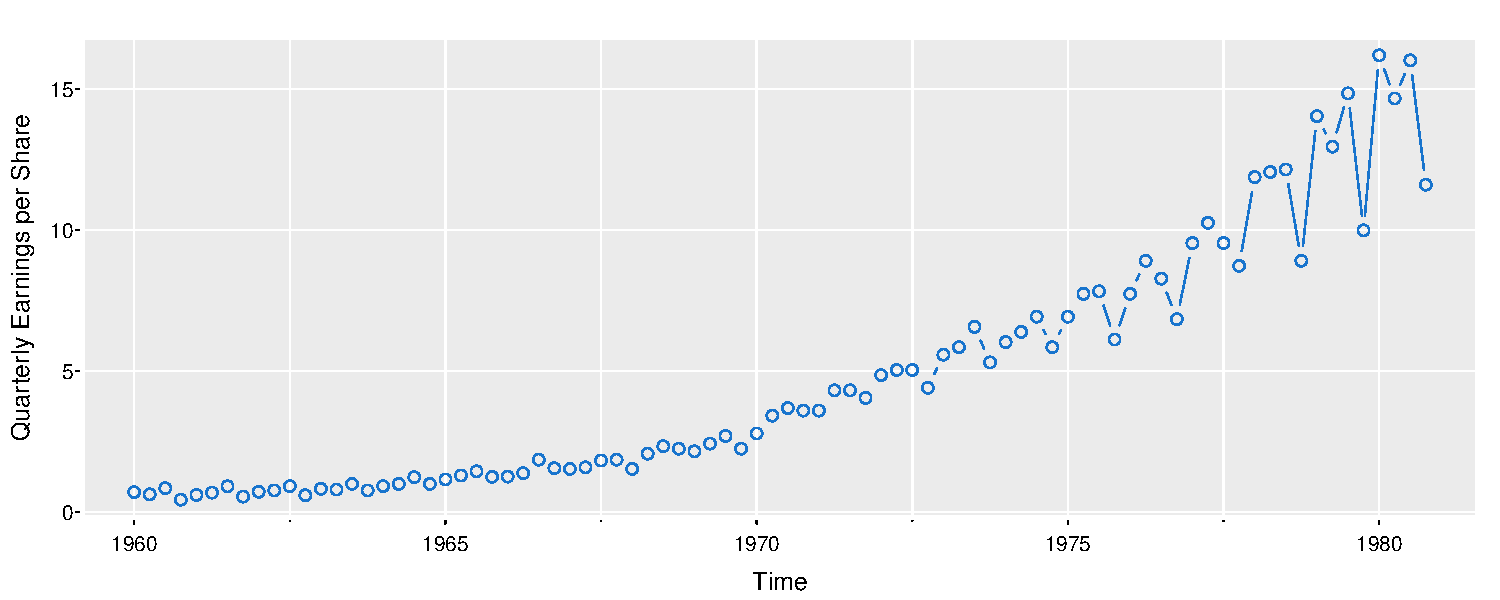
\includegraphics[width=.9\textwidth]{figure1.pdf}
\caption{Example of time series data}
\label{fig:figure1}
\end{figure}

At its core, a time series is a sequence of data points recorded at successive time intervals. The data is typically collected at uniform intervals -- be it hourly, daily, monthly, or yearly. Time series analysis helps in understanding the inherent structure and functions that generate the series. It aims to model the underlying context of the data, whether to understand the past behavior or to forecast future values.

The analysis of time series can be divided broadly into two types: descriptive and inferential. Descriptive analysis focuses on visualizing and summarizing the main features of the data, such as trends (long-term direction), seasonality (regular pattern of fluctuation within a year), and irregular components (unpredictable, random fluctuations). Inferential analysis, on the other hand, involves using models to predict future values based on known past values, testing hypotheses, and deriving estimates of population parameters.

In time series analysis, two fundamental approaches to examining data are the time-domain and the frequency-domain approaches. The \emph{time-domain approach} analyzes data as it evolves over time, focusing on the relationship between current and past values to predict future values. This approach is primarily concerned with understanding and modeling the temporal sequence directly in the time dimension. This approach is particularly useful for forecasting, where understanding how values are correlated through time is essential. It provides direct and often simple models that are interpretable in terms of the original time series data.

The \emph{frequency-domain approach}, on the other hand, analyzes data based on the rate at which the data's features repeat over time. This approach transforms the time series data into the frequency domain using mathematical transformations (the most common being the Fourier Transform). It decomposes the time series into a combination of sinusoid functions with different frequencies and amplitudes. The frequency-domain approach is useful for identifying hidden periodicities or cyclical behaviors in the data, which may not be apparent in the time domain.

\section{Time Series Statistical Models}

Time series statistical models are essential tools used to analyze and forecast time-dependent data. Four common models are the moving average (MA) model, the autoregressive (AR) model, the random walk with drift, and the signal in noise model. Each model has different characteristics and applications, suited to different types of time series data.

\subsubsection*{Moving Average Model}

The \emph{Moving Average} model is a fundamental time series model that expresses the current value of the time series as a function of past errors or deviations, with the assumption that these errors are white noise, that is, random. An example model is given by: 

\begin{align*}v_t = \frac{1}{3} ( w_{t-1} + w_t + w_{t+1})
\end{align*}

\noindent where $w_t$ are the white noise error terms. In this example, all white noise terms are weighted equally by $1/3$.

MA models are particularly useful in smoothing out noise and forecasting when the series exhibits a random behavior with no trend or seasonality.

The following R code block uses the \texttt{filter} function to generate the example model. The filter operates on the white noise, extending to both sides of the current time step, and creates a weighted sum of the closest three value in \texttt{w}, specified by the \texttt{mode='convolution'} argument. The resulting plots are shown in Figure~\ref{fig:figure2}. 

\begin{samepage}
\begin{Rcode}
# Random numbers as errors
w <- rnorm(500,0,1)
# Moving average
v <- filter(w, sides=2, filter=c(1/3,1/3,1/3), method='convolution')
# Plot timeseries
par(mfrow=c(2,1))
# The astsa library contains the tsplot function
library(astsa)
tsplot(w, main="white noise", col=3, gg=T)
tsplot(v, ylim=c(-3,3), main="moving average", col=4, gg=T)
\end{Rcode}
\end{samepage}

\begin{figure}
\centering

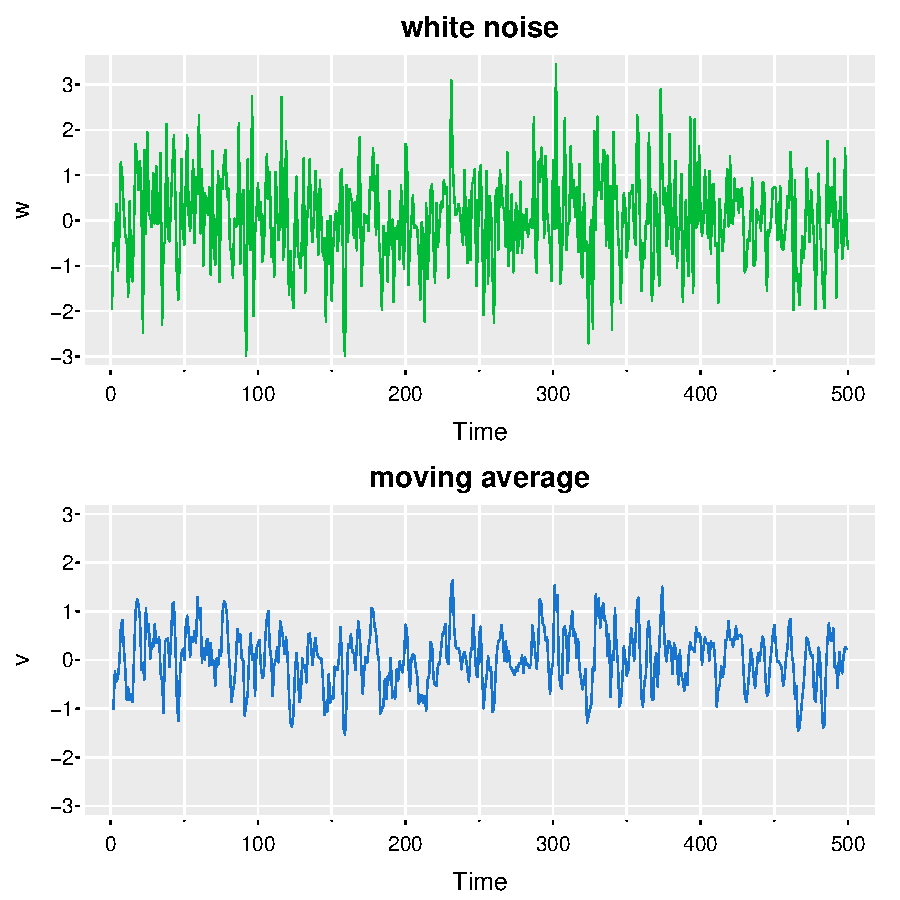
\includegraphics[width=.75\textwidth]{figure2.pdf}
\caption{Example white noise time series and its moving average}
\label{fig:figure2}
\end{figure}

\subsubsection*{Autoregressive Model}

The \emph{Autoregressive (AR) model} is based on the concept that current values of a series can be forecasted from previous values. An example model is:

\begin{align*}x_t = x_{t-1} - 0.9 x_{t-2} + w_t\end{align*}


\noindent where $w_t$ is white noise.

AR models are widely used in economic and financial time series where data points are influenced significantly by their previous values.

The following R code uses the \texttt{filter} function in ''recursive'' mode with parameters \texttt{1} and \texttt{-.9} to create the time series corresponding to the example model\footnote{The R code for this and following examples are based on material Shumway \& Stoffer}. The resulting plot is shown in Figure~\ref{fig:figure3}.

\begin{Rcode}
# Random numbers (errors)
w <- rnorm(550,0,1)
# remove first 50 values for startup
x <- filter(w, filter=c(1,-.9), method="recursive")[-(1:50)]
tsplot(x, main="autoregression", col=4, gg=T)
\end{Rcode}

\begin{figure}
\centering

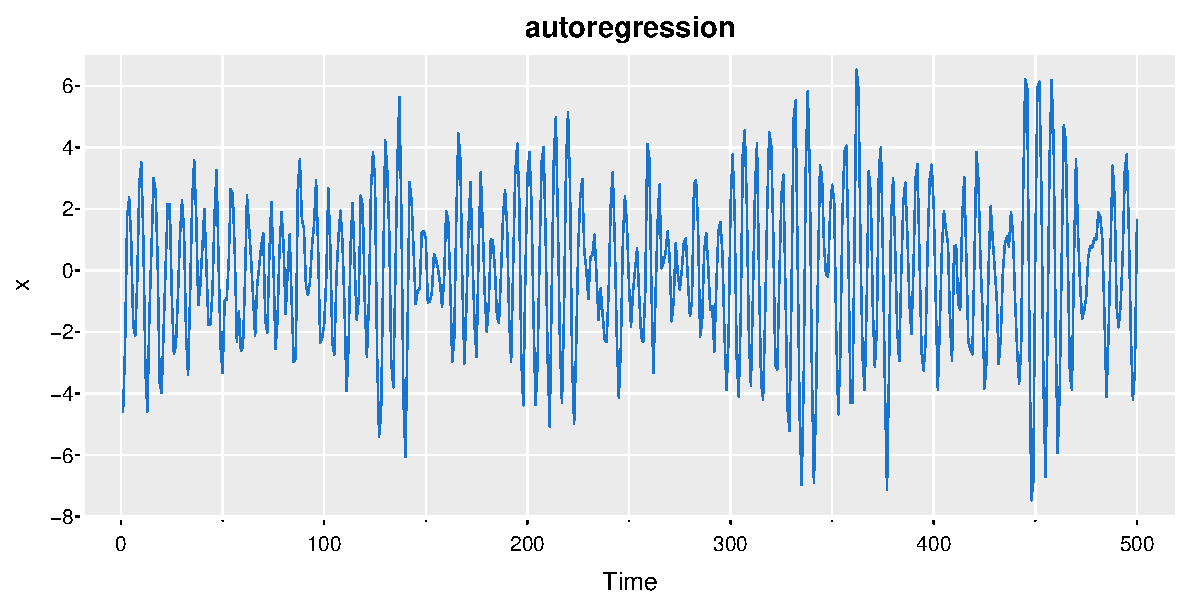
\includegraphics[width=.75\textwidth]{figure3.pdf}
\caption{Example autoregressive time series}
\label{fig:figure3}
\end{figure}

\subsubsection*{Random Walk with Drift}

A \emph{random walk with drift} adds a constant to the standard random walk, allowing the series to drift upwards or downwards over time. An example model is given by:

\begin{align*}x_t &= \delta + x_{t-1} + w_t \\
&= \delta t + \sum_{j=1}^t w_j
\end{align*}

\noindent where $\delta$ represents the drift (constant term), and $w_t$ is the noise component.

This model is commonly applied in financial markets to model stock prices or other investments, reflecting that prices are serially correlated and can trend over time.

The following R code block uses the the \texttt{cumsum()} function to calculate the cumulative sum. The resulting time series are shown in Figure~\ref{fig:figure4} and show the random walk and the drift component that is added to it.

\begin{samepage}
\begin{Rcode}
# Create random walk (white noise) model and then add drift
w <- rnorm(200)
x <- cumsum(w)
drift <- .2
w.drift <- w + drift;
x.drift <- cumsum(w.drift)
# Plot the two resulting series
tsplot(x.drift, ylim=c(-10,55), main="random walk",ylab='',col=3,gg=T)
abline(a=0, b=drift, lty=2, col=3)
lines(x, col=4)
abline(h=0, col=4, lty=2)
\end{Rcode}
\end{samepage}

\begin{figure}
\centering
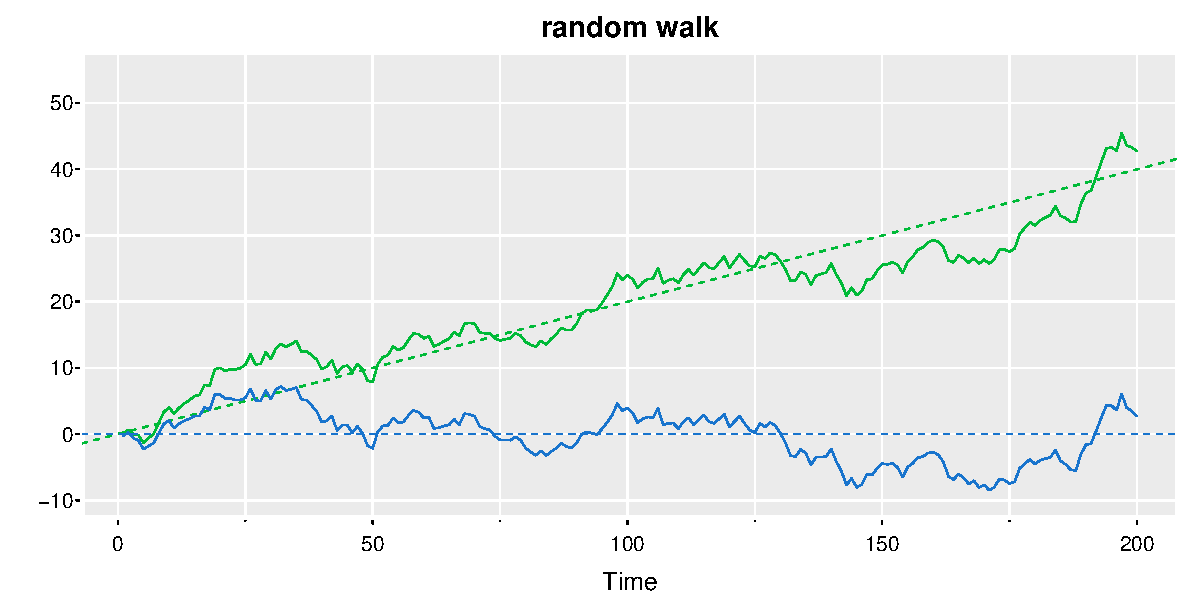
\includegraphics[width=.75\textwidth]{figure4.pdf}
\caption{Example random walk with drift time series}
\label{fig:figure4}
\end{figure}

\subsubsection*{Signal in Noise Model}

The \emph{Signal in noise} model views the time series as a combination of a true signal and random noise. An example model with a sinusoidal signal characterized by its amplitude, frequency and phase shift is:

\begin{align*}
x_t &= A \cos (2 \pi \omega t + \phi) 
\intertext{for example,}
A &= 2 &\qquad \text{amplitude} \\
\omega &= 1/50 &\qquad \text{frequency} \\
\phi &= .6 \pi &\qquad \text{phase shift}
\end{align*}

This model is fundamental in signal processing and is used to understand underlying trends in the presence of noisy observations. Techniques like filtering and smoothing are often applied to extract the signal from $x_t$.

The following R code block creates a sinusoidal signal and overlays it with different amounts of white (Gaussian) noise. The resulting time series are shown in Figure~\ref{fig:figure5}.

\begin{Rcode}
# Create signal
cs = 2*cos(2*pi*1:500/50 + .6*pi)
w = rnorm(500,0,1)
# Overlay with gaussian noise and plot
par(mfrow=c(3,1), mar=c(3,2,2,1), cex.main=1.5)
tsplot(cs, main='Signal', col=2, gg=T)
tsplot(cs+w, main='Signal and N(0,1) noise', col=3, gg=T)
tsplot(cs+5*w, main='Signal and N(0,25) noise', col=4, gg=T)
\end{Rcode}

\begin{figure}
\centering
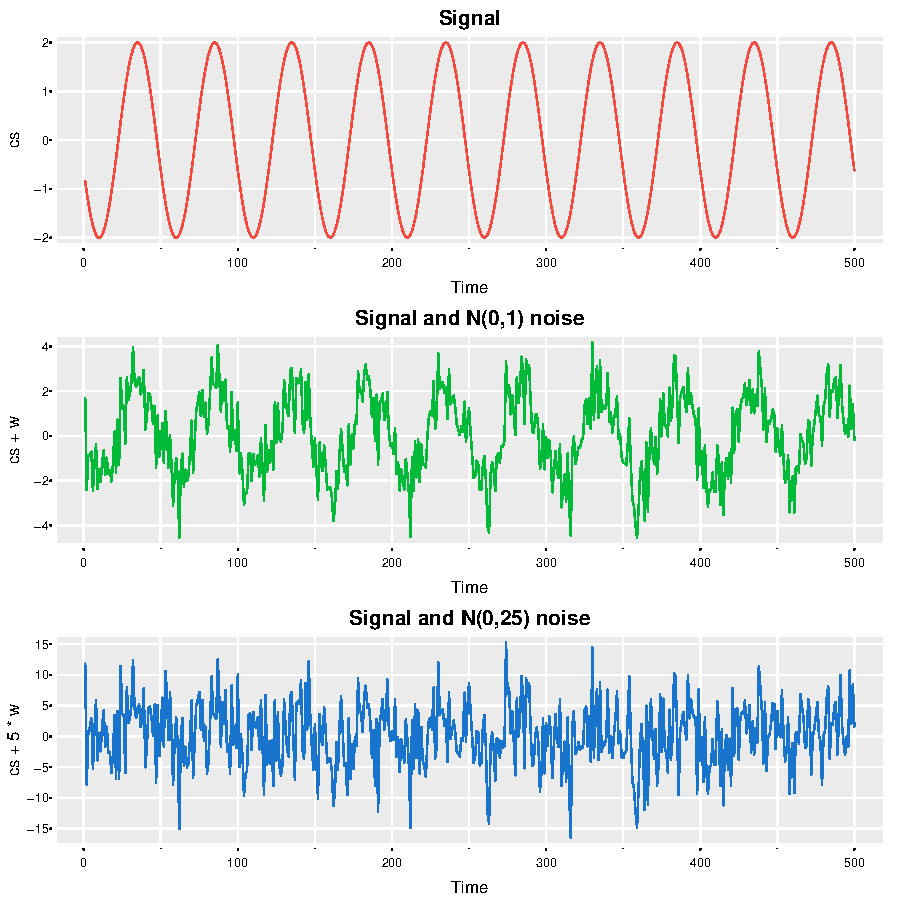
\includegraphics[width=.75\textwidth]{figure5.pdf}
\caption{Example signal in noise time series}
\label{fig:figure5}
\end{figure}

\section{Basic Time Series Operations in R}

A time series can be constructed from an ordinary data set using the \texttt{ts()} function in R and supplying a start time stamp and a sampling frequency. For example, the following R code creates a time series of montly observations, beginning in January 2020 with the values 1 through 24. R will try to sensibly interpret the \texttt{start} and \texttt{frequency} arguments: Frequencies of 4 are interpreted as quarters of the year, 7 is interpreted as days of a week, 12 is interpreted as months of the year.

\begin{samepage}
\begin{Rcode}
# Creating a time series object with monthly data
ts_data <- ts(1:24, frequency = 12, start = c(2020, 1))
\end{Rcode}
\end{samepage}

\noindent To see the first and last last observations of a time series, use the \texttt{head()} and \texttt{tail()} functions:

\begin{samepage}
\begin{Rcode}
head(ts_data)
tail(ts_data)
\end{Rcode}
\end{samepage}

Missing values in a time series cannot be imputed in the usual manner because the observations are not independent of each other. Two simple ways of ''filling in'' missing data are either to simply carry the last observation forward, which assumes there are negligible changes in the value over time, or to interpolate the missing values. In linear interpolation, a line is imagined between the last observation before a series of missing values and the first observation after such a series of missing values. Missing values are then assumed to be on that line. This assumes that the time series is approximately linear, at least for short gaps. 

The \texttt{zoo} library for R contains the functions \texttt{na.locf()} and \texttt{na.approx()} that implement these methods of handling missing values. Missing values at the beginning or end of a time series can be removed with the \texttt{na.trim()} function. The following R code block illustrates the use of all three functions:

\begin{samepage}
\begin{Rcode}
# Introduce NA values into the time series
ts_data[c(5, 10, 15)] <- NA

# Using na.trim to remove leading/trailing NA values
trimmed_ts <- na.trim(ts_data)
# Using na.locf (Last Observation Carried Forward) to handle NA values
locf_ts <- na.locf(ts_data)
# Using na.approx to interpolate NA values
approx_ts <- na.approx(ts_data)
\end{Rcode}
\end{samepage}

Two time series can be combined using the \texttt{ts.intersect()} or \texttt{ts.union()} functions. The former function combines the series only for overlapping, that is, intersecting, times, possibly cutting off the head or tail of one or the other series. The latter function retains all dates of both series and ''pads'' the head or tail of one or the other series with ''NA'' values. 

\begin{samepage}
\begin{Rcode}
# Creating another time series
ts_data2 <- ts(c(1:24), frequency = 12, start = c(2020, 7))

# Using ts.intersect to determine intersection of two time series
intersect_ts <- ts.intersect(ts_data, ts_data2)
# Using ts.union to determin union of two time series
union_ts <- ts.union(ts_data, ts_data2)
\end{Rcode}
\end{samepage}

An important operation in time series analysis is to ''lag'' a time series, that is, to shift it forwards or backwards in time. R provides the \texttt{lag()} function for this purpose. A positive argument shifts the time series \emph{backwards} by the specified number of time periods, while a negative argument shifts it forward:

\begin{samepage}
\begin{Rcode}
# Positive k shifts backwards in time
lag_ts <- lag(ts_data, 2)
# Negative k shifts forwards in time
lag_ts <- lag(ts_data, 3)
\end{Rcode}
\end{samepage}

\section{Smoothing a Time Series}

Time series smoothing is a technique used to remove noise and reveal signals or underlying trends in the data. Four commonly used methods for time series smoothing are moving average, kernel smoothing, lowess regression, and smoothing splines. 

\subsubsection*{Moving Average Smoothing}

\emph{Moving average smoothing} is one of the simplest and most widely used methods for smoothing time series data. It involves calculating the weighted mean of the consecutive data points within a specified window that moves along with the data:

\begin{align*}m_t = \sum_{j=-k}^k a_j x_{t-j} \quad \text{where} \quad
\sum_{j=-k}^k a_j = 1
\end{align*}

\noindent where $a$ are the weights that sum to one. A simple filter uses uniform weights, but other shapes are possible.

This model can be implemented using the \texttt{filter} function in R. The filter in the example below is two-sided and is centered on the current time stamp, that is, it uses data before and after the current time point. When the \texttt{sides=1} argument is used, the filter is over past values only. The \texttt{filter} argument specifies the weights for the moving average. The results for an example time series are shown in Figure~\ref{fig:figure14}.

\begin{samepage}
\begin{Rcode}
# Use the soi dataset from the astsa library as an example
library(astsa)
?soi
# Apply moving average filter
f = 1/12 * c(0.5, 1, 1, 1, 1, 1, 1, 1, 1, 1, 1, 1, 0.5)
filter(soi, sides=2, filter=f, method='convolution')
\end{Rcode}
\end{samepage}

\begin{figure}
\centering
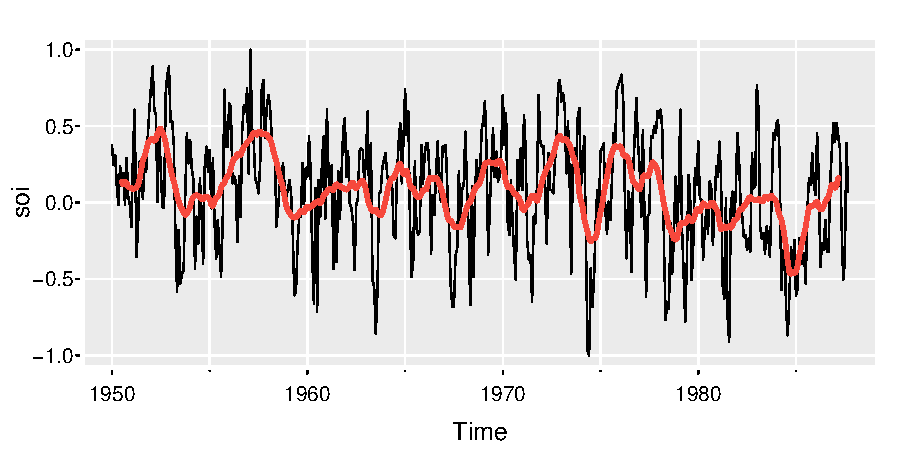
\includegraphics[width=.75\textwidth]{figure14.pdf}
\caption{Moving average smoothing}
\label{fig:figure14}
\end{figure}

\subsubsection*{Kernel Smoothing or Kernel Regression}

Instead of a filter with simple weights as in moving average smoothing, \emph{kernel smoothing} uses a weighted average of neighbouring points where the weights are determined by a function known as the \emph{kernel}. A common choice is a Gaussian kernel that uses the normal distribution density function, which produces a weighted average with a bell-shaped curve of weights around each data point. The weights for averaging the time series values are determined as follows:

\begin{align*}
a_i(t) &= \frac{K\left(\frac{t-i}{b}\right)}{\sum_{j=1}^n K \left(\frac{t-j}{b}\right) }
\intertext{where $K$ is the Gaussian kernel:}
K(z) &= \frac{1}{\sqrt{2\pi}} \exp(-z^2/2) 
\end{align*}

Here, $b$ is the ''bandwidth'' of the kernel, that determines the shape of the kernel function, that is, how ''wide'' or ''broad'' it is.

The smoothed time series $s_t$ is then given by:

\begin{align*}
s_t &= \sum_{i=1}^n a_i(t) x_t \\
 &= \frac{\sum_{i=1}^n K\left(\frac{t-i}{b}\right) x_t}{\sum_{j=1}^n K \left(\frac{t-j}{b}\right) }
\end{align*}


\noindent The R function \texttt{ksmooth()} with the \texttt{normal} kernel argument provides exponential smoothing. The \texttt{bandwidth} parameter determines the ''width'' of the kernel by specifying the distance from the quartiles to the mean of the normal distribution function. Example smoothing results for various bandwidth values are shown in Figure~\ref{fig:figure15}.

\begin{Rcode}
# Apply gaussian kernel smoothing
ksmooth(time(soi), soi, kernel='normal', bandwidth=1)
\end{Rcode}

\begin{figure}
\centering
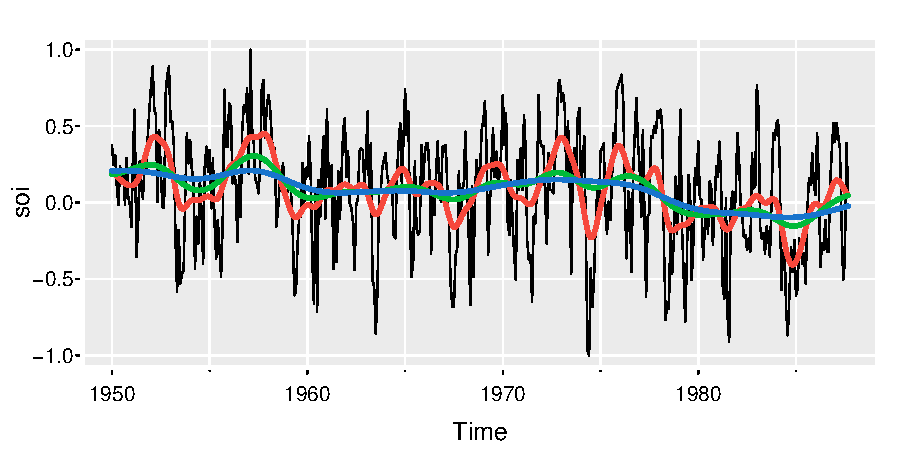
\includegraphics[width=.75\textwidth]{figure15.pdf}
\caption{Kernel density smoothing with different kernel bandwidths}
\label{fig:figure15}
\end{figure}

\subsubsection*{Lowess Regression}

\emph{Lowess Regression} (locally weighted scatterplot smoothing) combines a multiple regression model with a k-nearest-neighbour-based model. Each point on the smoothed time series is estimated by a weighted least squares regression over a local neighbourhood of $f$ observations that are closest in time to the target point. The weights decrease with distance from the target observation, thereby providing robustness against outliers and yielding a smooth curve that closely follows the data. 

The R function \texttt{lowess()} uses the \texttt{f} parameter for specifying the proportion of observations used for the regressions. An example result is shown in Figure~\ref{fig:figure16}.

\begin{Rcode}
# Apply lowess smoothing
lowess(soi, f=0.1)
\end{Rcode}

\begin{figure}
\centering
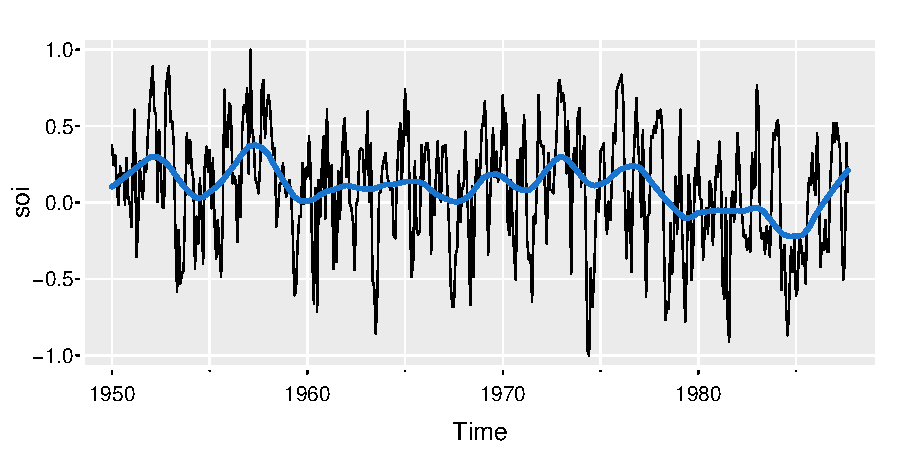
\includegraphics[width=.75\textwidth]{figure16.pdf}
\caption{Lowess regression smoothing example}
\label{fig:figure16}
\end{figure}

\subsubsection*{Smoothing Splines}

\emph{Smoothing splines} are a method that fits a smooth, flexible ''spline'' function to the data. Smoothing splines balance the fit of the spline to the data against the smoothness of the spline curve and are essentially penalized polynomial regression models that fit the model:

\begin{align*}
m_t = \beta_0 + \beta_1 t + \beta_2 t^2 + \beta_3 t^3
\intertext{by minimizing the loss function}
\sum_{t=1}^n (x_t - m_t)^2 + \lambda \int \left( \dv[2]{m}{t} \right)^2 \, dt
\end{align*}

The \texttt{smooth.spline()} function uses cubic splines, that is polynomials of degree $3$. The smoothing parameter \texttt{spar} controls the regression penalty $\lambda$ in the equation above and thereby the degree of smoothing. The result for this example is shown in Figure~\ref{fig:figure17}.

\begin{Rcode}
# Apply smoothing splines
smooth.spline(time(soi), soi, spar=0.5)
\end{Rcode}


\begin{figure}
\centering
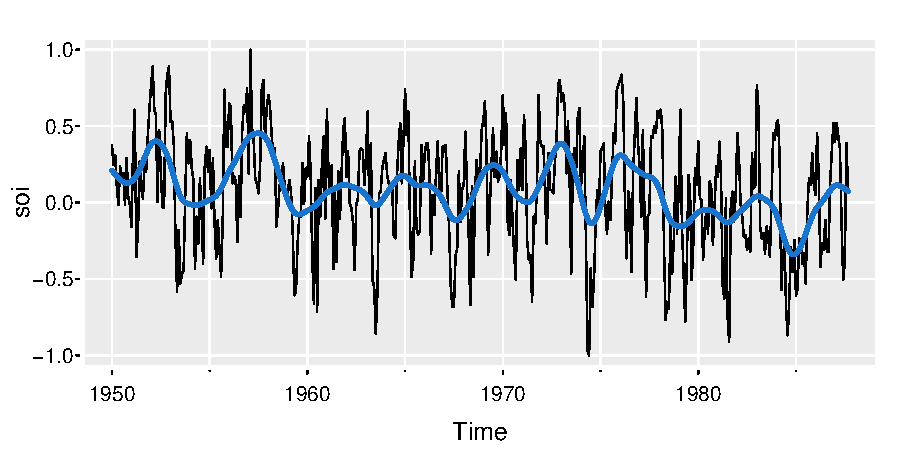
\includegraphics[width=.75\textwidth]{figure17.pdf}
\caption{Smoothing spline example}
\label{fig:figure17}
\end{figure}

\begin{tcolorbox}[colback=code]
\subsubsection*{Hands-On Exercise} 
\begin{enumerate}
\item Generate 100 observations from the autoregression model $x_t = -.9x_{t-2} + w_t$ with $\sigma^2_w = 1$
\begin{enumerate}
   \item Smooth the time series using a moving average filter $v_t = (x_t + x_{t-1} + x_{t-2} + x_{t-3})/4$, plot $x_t$ as a line and superimpose $v_t$. Comment on the behaviour of $x_t$ and how applying the moving average filter changes that behavior
   \item Smooth the time series using kernel smoothing, produce plots as above, and experiment with different kernel bandwidths. Comment on the behvaiour of the smoothed series.
   \item Smooth the time series using Lowess, produce plots as above, and experiment with different values for the fraction of observations to include in each regression. How does the smoothed series change as you vary that fraction?
   \item Smooth the time series using smoothing splines, produce plots as above, and experiment with different values for the smoothing parameter that controls the regression penalty. How does the smoothed series change as you vary that parameter?
\end{enumerate}

\item Generate 100 observations from the sinusoidal series $x_t = \cos(2 \pi t / 4)$ and add $N(0,1)$ noise. Repeat the four smoothing exercises. Compare and contrast the results of these exercises. Which smoothing is more appropriate for which type of time series data?
\end{enumerate}
\end{tcolorbox}

\section{Time Series Regression}

Time series regression refers to using time series data in ordinary least squares regression. The focus is not necessarily on modeling data series over time or describing the future values of a time series as a function of earlier values, although lagged time series can certainly be used in time series regression. Instead, time series regression predicts the value of one time series from one or more other time series. 

Consider an epidemiological example with three weekly time series, one expressing cardiovascular mortality (''cmort'', the likelihood of dying of heart attack), another describing ambient temperature (''tempr'') and a third one describing air pollution (''part''). Figure~\ref{fig:figure11} shows these three time series superimposed in one graph. Visual inspection of the graph suggests that mortality may be correlated with temperature and air pollution.

\begin{figure}
\centering
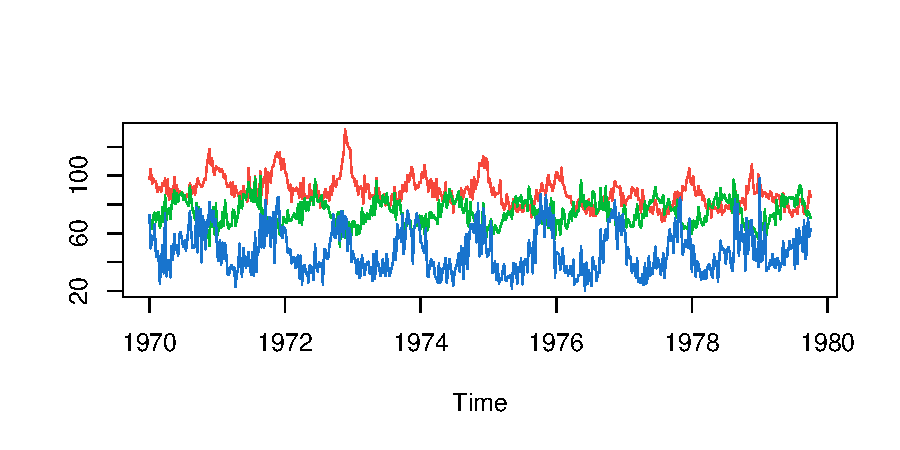
\includegraphics[width=.9\textwidth]{figure11.pdf}
\caption{Three time series}
\label{fig:figure11}
\end{figure}

Time series regression uses ordinary least squares (OLS) regression models where each series is a predictor variable. It essentially neglects the time aspect of the time series data. The following R code block shows examples of time series regression to predict or explain mortality. Note the use of the \texttt{time()} function extract the timestamps from the time series data.

\begin{samepage}
\begin{Rcode}
# Use data from the astsa library
library(astsa)
# Plot the three time series
ts.plot(cmort, tempr, part, col=2:4)
# Center the temperature variable
temp = tempr - mean(tempr)
# Square the temperature variable
temp.2 = temp^2
# Fit different linear models and provide summaries
summary(lm(cmort ~ time(cmort)))
summary(lm(cmort ~ time(cmort) + temp))
summary(lm(cmort ~ time(cmort) + temp + temp.2))
summary(lm(cmort ~ time(cmort) + temp + temp.2 + part))
\end{Rcode}
\end{samepage}

Time series regression can also use lagged time series data, that is, data of the same series that is shifted backward in time. This is somewhat similar to the autoregressive models defined below. The following R code block lags the temeratur by two weeks and by four weeks. It then uses \texttt{ts.intersect()} to combine the time series in a data frame for the times where they intersect. The data frame is then be used in an OLS regression; different models could be fitted to identify the best explanation of mortality.

\begin{samepage}
\begin{Rcode}
# Lag the temperature
temp.l.2 = lag(temp, 2)
temp.l.4 = lag(temp, 4)
# Intersect all time series to omit leading/trailing NA
temp.df <- ts.intersect(cmort, time(cmort), part, 
                  temp, temp.2, temp.l.2, temp.l.4, dframe=TRUE)
# Fit the linear model including lagged temperature
summary(lm(cmort ~ time.cmort. + temp + temp.2 + 
                      temp.l.2 + temp.l.4 + part, data=temp.df))
\end{Rcode}
\end{samepage}

\section{Stationarity}

The concept of \emph{stationarity} is central to time series analysis. Stationarity means that the statistical characteristics of a time series do not change over time. That is, its mean, variance, and autocorrelation (the correlation of a time series with a lagged copy of itself) remain constant over time. Understanding and ensuring stationarity in a time series is important for the effective application of many statistical forecasting methods and models.

Stationary data with a constant mean and variance is more predictable and therefore easier to model. Changes in mean and variance can lead to forecasts that are biased or that degrade in accuracy over time. Stationarity ensures that the properties of the series used to generate forecasts will be similar in the future, which is crucial for planning and decision-making. If a time series is non-stationary, the behavior of the data could change over time, leading to models that are invalid or inaccurate when applied to future data points.

Statistical inference in time series analysis relies heavily on the assumption of stationarity. Many time series statistical models, including linear regression and ARMA models, are based on the assumption of stationarity. These models provide meaningful and reliable results only if the stationarity assumption is satisfied. 

\emph{Strict stationarity} is defined as the requirement that the probabilistic behaviour of every set of values of the series
\begin{align*}\{x_{t1}, x_{t2}, \ldots, x_{tk} \} \end{align*}
\noindent is identical to that of the set of values shifted by time $h$:
\begin{align*}
\{x_{t1+h}, x_{t2+h}, \ldots, x_{tk + h} \}
\end{align*}
\noindent That is,
\begin{align*}
&\Pr \{ x_{t1} \leq c_1, \ldots, x_{tk} \leq c_k \} = \Pr \{ x_{t1+h}\leq c_1, \ldots , x_{tk+h} \leq c_k \}
\end{align*}

Because strong stationarity is hard to test, a more commonly used and practical form of stationarity is \emph{weak stationarity}, which requires only that the the mean, variance, and the \emph{autocovariance} (the covariance of the series with a lagged version itself) are constant over time. Most statistical tests and models assume weak stationarity. In summary, a weakly stationary time series is a finite variance process such that:

\begin{enumerate}
\item The mean and variance are constant and do not depend on time: $\mu_t = \mu$, $\sigma_t = \sigma$
\item The autocovariance $\gamma$ depends on $s$ and $t$ only through their difference $h=|s-t|$.
\end{enumerate}

Let $s = t + h$, then under the assumption of weak stationarity:
\begin{align*}
\gamma(s, t) &= \gamma(t+h, t)  &\text{(because of condition 2)} \\ 
             &= cov(x_{t+h}, x_t)  &\text{(because of condition 1)} \\ 
             &= cov(x_h, x_0) = \gamma(h)  &\text{(autocovariance for lag $h$)} \\
\intertext{and}
\rho(h) &= \gamma(h) / \gamma(0) &\text{(autocorrelation for lag $h$)}
%\intertext{and the CCF of two jointly stationary time series is}
%\rho_{xy}(h) &= \frac{\gamma_{xy}(h)}{\sqrt{\gamma_x(0)\gamma_y(0)}}
\end{align*}

The \emph{autocovariance} and \emph{autocorrelations} are measures of dependence of the time series on lagged versions of itself. For a weakly stationary time series, the theoretical autocovariance for a lag $h$ is defined as the covariance between two points $t, t+h$ on time series $x$
\begin{align*}
\gamma(h) = cov(x, x_{t+h}) = E [ (x_t - \mu)(x_{t+h} - \mu)] 
\end{align*}

Note that this definition implies weak stationarity because a constant term for the mean $\mu$ is used in the expectation on the right-hand side.

A large autocovariance indicates a ''smooth'' time series, as each future value is strongly dependent on the previous value(s). In contrast, a small autocovariance indicates the ''choppy'' time series, as there is less dependence on prior values and values of the time series are less constrained and allowed to vary more. 

The sample autocovariance that can be estimated from a finite sample for lag $h$ is defined as  

\begin{align*}
\hat{\gamma}(h)  = \frac{1}{n} \sum_{t=1}^{n-h} (x_t - \bar{x})(x_{t+h} - \bar{x})
\end{align*}

The \emph{autocorrelation function} (ACF) for lag $h$ is defined as usual as the autocovariance divided by the root of the product of the variances of the two time series:

\begin{align*}
\rho_x(h) = \frac{\gamma (t+h,t)}{\sqrt{\gamma (t+h,t+h) \gamma(t, t)}} = \frac{\gamma(h)}{\gamma(0)}  \quad \text{\small (weak stationarity)}
\end{align*}

Note that this assumes weak stationarity. The time series properties at any time $t$ are the same as at time $0$ so that the above equation can be reduced to the right-most term.

Similar to the sample autocovariance, the sample ACF for lag $h$ is defined as

\begin{align*}
\hat\rho_x(h) = \frac{\hat\gamma(h)}{\sqrt{\hat\gamma(h) \hat\gamma(0)}} = \frac{\hat\gamma(h)}{\hat\gamma(0)} \quad \text{\small (weak stationarity)}
\end{align*}

\noindent where the last step again assumes weak stationarity.

To test whether the ACF of any sequence for lag $h$ is statistically different from $0$, note that the large-sample distribution of $\hat{\rho}_{x}(h)$ is normal with mean $0$ and standard deviation
\begin{align*}
\sigma_{\hat{\rho}_{x}} = 1/ \sqrt{n} 
\end{align*}

\noindent if the generating processes is independent white noise. Hence, the approximate $95\%$ confidence interval on the ACF is
\begin{align*}
-\frac{1}{n} \pm \frac{2}{\sqrt{n}}
\end{align*}

If the sample ACF of $n$ values of a time series for a given lag exceeds the lower or upper bounds of the confidence interval, the ACF is statistically significantly different from $0$, and the time series is unlikely to be white noise.

The following R code block illustrates the autocorrelation function using the standard \texttt{cor()} function to compute the correlations at different lags and the \texttt{acf1()} function of the \texttt{astsa} library that will automatically lag the time series and output and optionally plot the ACF values at different lags, creating a plot as in Figure~\ref{fig:figure7a}.

\begin{figure}
\centering
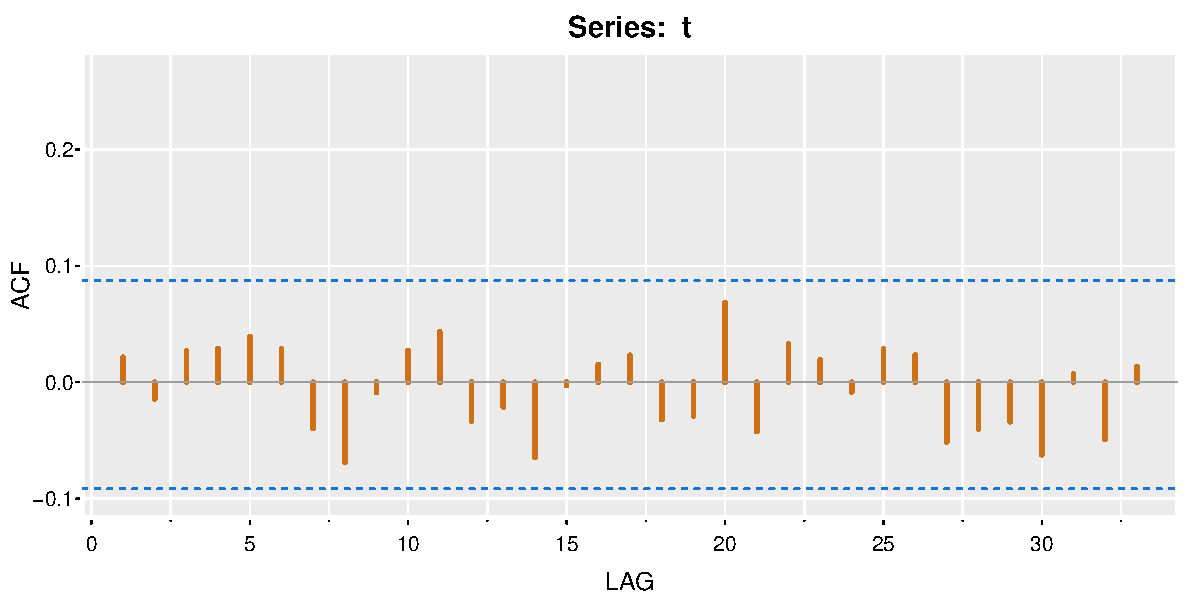
\includegraphics[width=.75\textwidth]{figure7a.pdf}
\caption{ACF of Gaussian white noise}
\label{fig:figure7a}
\end{figure}

\begin{samepage}
\begin{Rcode}
library(astsa)
# Create Gaussian white noise
t <- ts(rnorm(500))
# The hard way:
cor(ts.intersect(t, lag(t,1), dframe=T))
cor(ts.intersect(t, lag(t,2), dframe=T))
# etc.
# The easy way:
# Without plot
acf <- acf1(t, plot=FALSE)
# With plot
acf1(t, gg=T, col=7, lwd=3)
\end{Rcode}
\end{samepage}

The following example in R uses the \texttt{soi} data set and the \texttt{lag1.plot()} from the \texttt{astsa} library to provide also a graphical display of the autocorrelations at various lags, as shown in Figure~\ref{fig:figure8a}.

\begin{samepage}
\begin{Rcode}
library(astsa)
# Compute and plot the ACF for different lags
acf1(soi, gg=T, co=3, lwd=2)
# Scatterplot of original versus or lags up to 6, with ACF values
lag1.plot(soi, max.lag = 6, gg=T, col=4, lwl=3)
\end{Rcode}
\end{samepage}

\begin{figure}
\centering
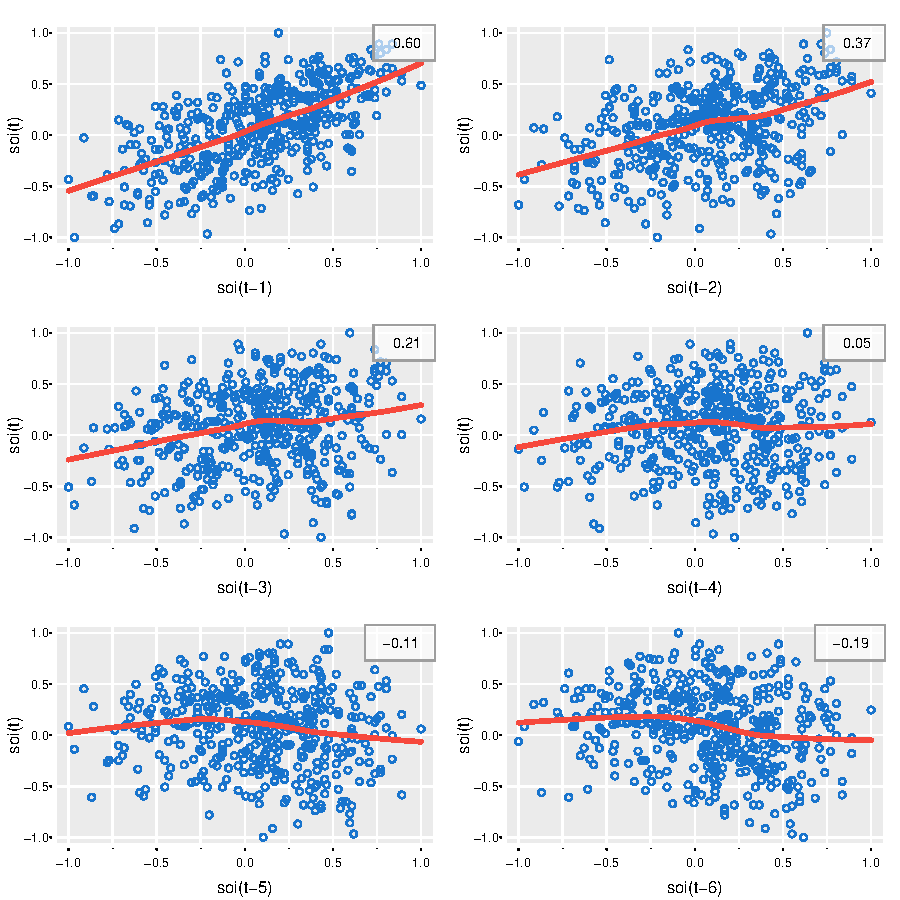
\includegraphics[height=3.75in]{figure8a.pdf}
\caption{Autocorrelations at six different lags}
\label{fig:figure8a}
\end{figure}

The \emph{partial autocorrelation function} (PACF) of a time series is a measure of the correlation between observations at two points in time, accounting for the correlations of the observations at all shorter intervals. Essentially, it reflects the direct effect of past data points on the future data point, after removing the effects of intermediate data points. PACF can be thought of as the correlation between a variable and its lag $h$ that is not explained by correlations at all lower-order lags. It is formally defined as the correlation between $x_{t+h}$ and $x_t$ with the linear dependence of $\{x_{t+1}, \ldots, x_{t+h-1}\}$ on each removed:

\begin{align*}
\phi_{hh} = \begin{cases}\rho(1) &\quad h = 1 \\
 \operatorname{corr}(x_{t+h} - \hat{x}_{t+h}, x_t - \hat{x}_t) &\quad h \geq 2
 \end{cases}
\end{align*}

The following R code block illustrates the use of the partial autocorrelation function of a time series, first using the standard \texttt{cor()} function for a lag of $3$ and then the \texttt{acf1()} function of the \texttt{astsa} library that automatically computes the PACF for different lags.

\begin{samepage}
\begin{Rcode}
t <- ts(rnorm(500))
# The hard way
# Shift the series to create lagged versions
t1 <- lag(t, 1)
t2 <- lag(t, 2)
t3 <- lag(t, 3)
data <- ts.intersect(t, t1, t2, t3, dframe=T)

# Using linear models to adjust for intervening lags
model_lag1 <- lm(t ~ t1 + t2, data)
model_lag2 <- lm(t1 ~ t2, data)
# Residuals for lag 3
residuals_lag1 <- residuals(model_lag1)
residuals_lag2 <- residuals(model_lag2)
final_model <- lm(residuals_lag1 ~ residuals_lag2)
# Correlation between residuals and lag 3 data
pacf_lag3 <- cor(residuals(final_model), data$t3)

# The easy way
acf1(t, plot=F, pacf=T)
\end{Rcode}
\end{samepage}

\section{Dealing with Non-Stationarity}

When a time series is non-stationary, it can often be transformed into a stationary series through techniques such as logarithmic or square root transformations, detrending, and differencing. These transformations can stabilize the mean and reduce variance dependency over time.

\subsubsection*{Transformations}

Popular \emph{time series transformations} are the log transformation, the square root transformation and the Box-Cox power transformation, defined as follows:

\begin{align*}y_t &= \log x_t \qquad \qquad \qquad \qquad \qquad \text{Log transformation}\\
  y_t &= \sqrt{x_t} \qquad \qquad \; \; \qquad \qquad \qquad \text{Square root transformation} \\
  y_t &= \begin{cases}(x_t^\lambda-1)/\lambda &\quad \lambda\neq0 \\
  \log x_t &\quad \lambda=0
  \end{cases} \qquad \text{Box-Cox power transformation}
\end{align*}

\subsubsection*{Detrending}

\emph{Detrending} a time series involves removing the trend component from the data, thereby isolating the non-trend components such as seasonality and irregular fluctuations. This is particularly useful in time series analysis because many statistical methods assume stationarity (constant mean and variance), and a trend violates these assumptions.

A common detrending method is to fit a regression model to the trend component and then subtract the fitted values, that is, the trend, from the original series. Linear regression is widely used for linear trends, but polynomial or more complex models can be fitted depending on the nature of the trend.

For example, assume that 
\begin{align*}
x_t = \mu_t + y_t
\end{align*}

where $\mu_t$ is the trend and $y_t$ a stationary series. Then detrending comprises the following two steps:

\begin{enumerate}
  \item Estimate trend, e.g. with a linear model such as $\mu_t = \beta_0 + \beta_1 t$
  \item Work with residuals, e.g. $\hat y_t = x_t - \hat \mu_t = x_t - \hat\beta_0 - \hat\beta_1 t$
\end{enumerate}

The following R code block shows how to detrend a time series using linear regression, producing the graphs shown in Figure~\ref{fig:figure39a}.

\begin{samepage}
\begin{Rcode}
# Simulate a time series with a linear trend
t <- ts(1:100 + rnorm(100) * 10)

# Fit a linear model to the time series
trend_model <- lm(t ~ time(t))
# Calculate detrended series by subtracting the estimated trend
detrended_series <- residuals(trend_model)

# Plot original and detrended
par(mfrow=c(2,1))
tsplot(t, type="l", main="original",col=3,gg=T)
tsplot(detrended_series, type="l", main="detrend",col=2,gg=T)
\end{Rcode}
\end{samepage}

\begin{figure}
\centering
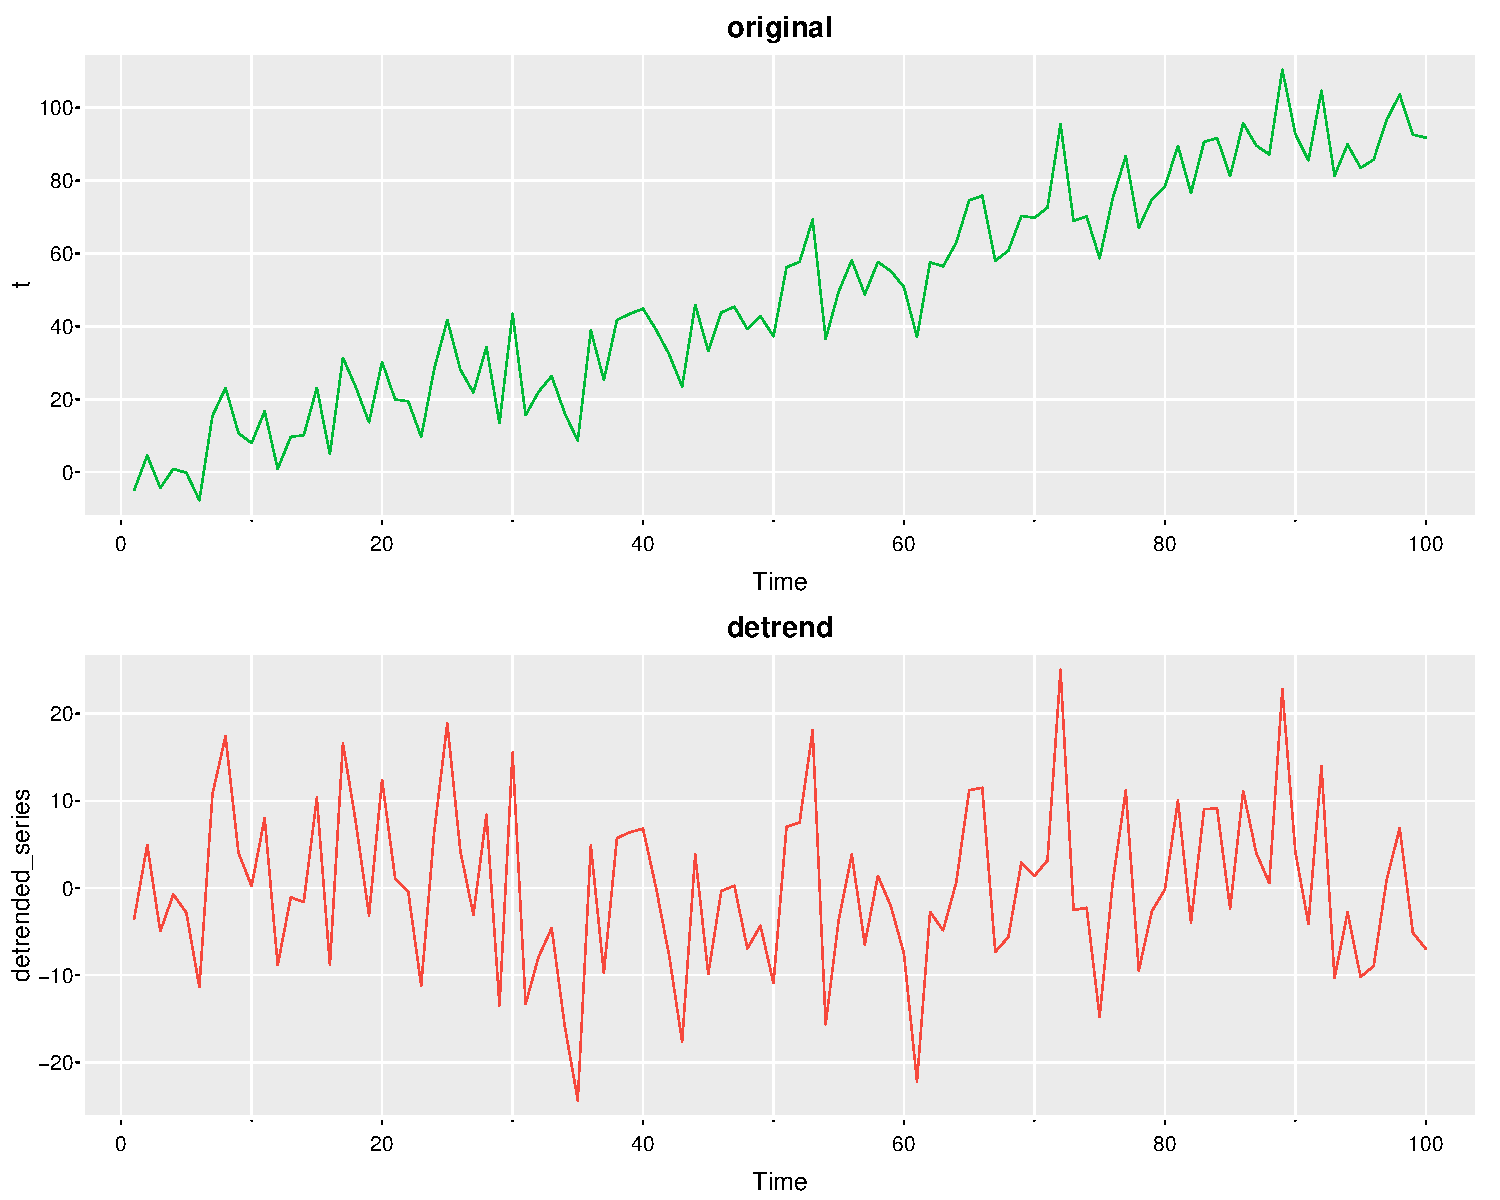
\includegraphics[width=.75\textwidth]{figure39a.pdf}
\caption{Time series and detrended time series}
\label{fig:figure39a}
\end{figure}

\subsubsection*{Differencing}

\emph{Differencing} involves computing the differences between consecutive observations in the original time series. The primary goal of differencing is to remove trends and seasonality in order to stabilize the mean of the time series by reducing changes in the level of a time series over time. Assume again that 

\begin{align*}x_t = \mu_t + y_t\end{align*}

\noindent where $\mu_t$ is the trend and $y_t$ a stationary series. Differencing models the trend stochastically as a random walk with drift: 

\begin{align*}\mu_t = \delta + \mu_{t-1} + w_t\end{align*}

\noindent where $w_t$ is white noise. Differencing then yields 
\begin{align*}
x_t - x_{t-1} &= (\mu_t + y_t) - (\mu_{t-1} + y_{t-1}) \\
 &= \delta + w_t + y_t - y_{t-1}
 \end{align*}
\noindent which is stationary.

As seen above, the first difference can remove a linear trend. However, sometimes the first difference is not enough to achieve stationarity. In such cases, the second difference can be used to remove a quadratic trend and higher-order differences can be computed if the series still shows non-stationary behavior after the second differencing.

The following R code shows the effect of differencing on a simulated time series. Differencing uses the \texttt{diff()} function. The resulting plots are shown in Figure~\ref{fig:figure40a}.

\begin{figure}
\centering
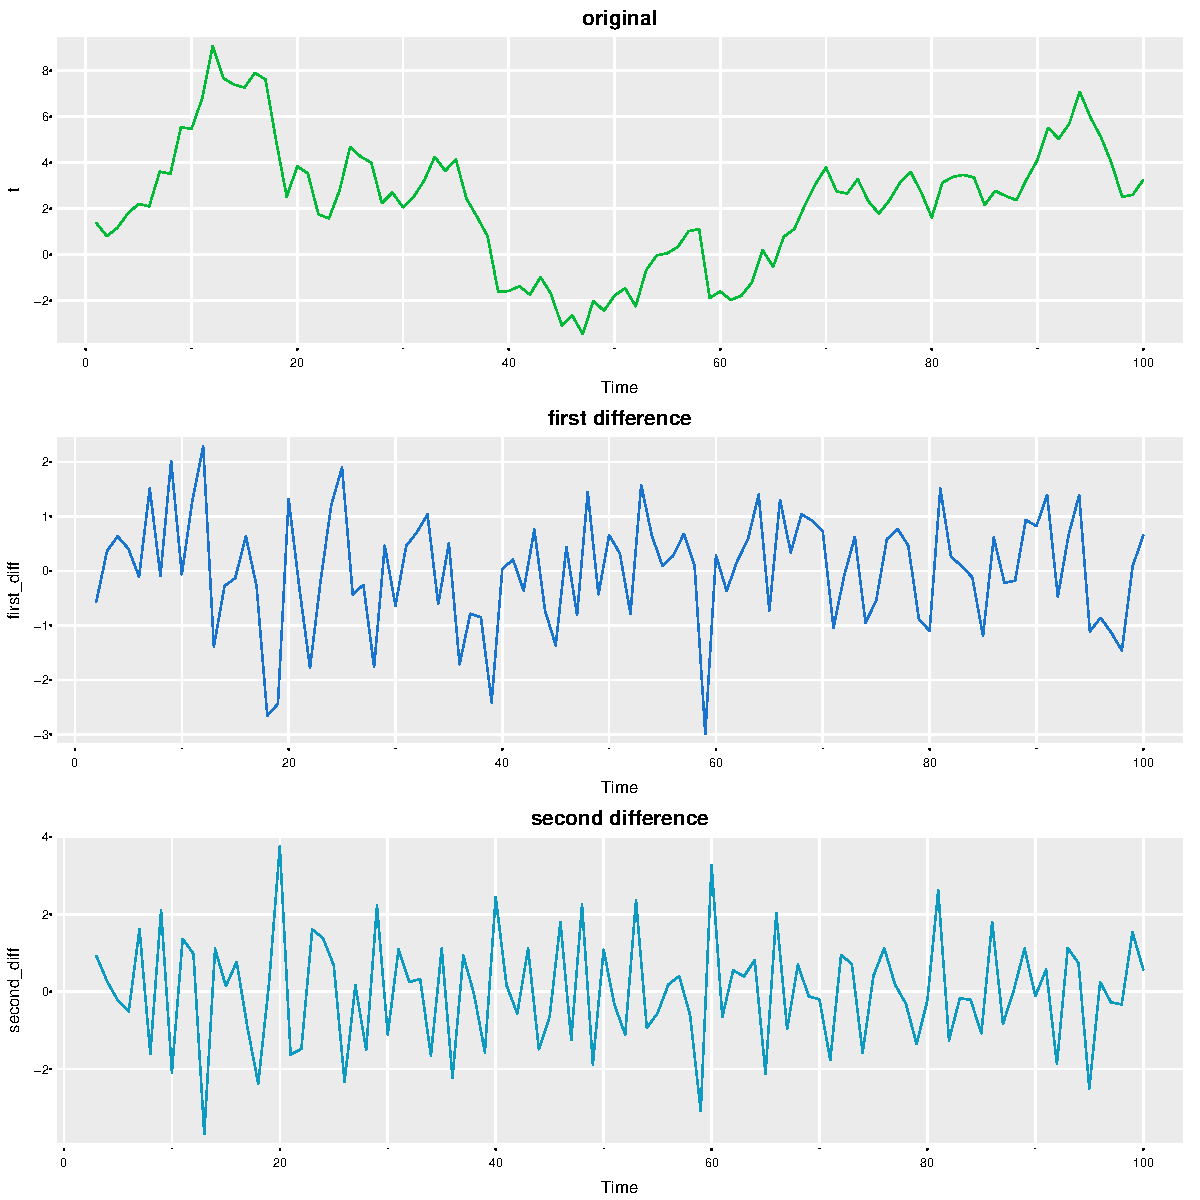
\includegraphics[width=.75\textwidth]{figure40a.pdf}
\caption{Original, first and second differences of a simulated time series}
\label{fig:figure40a}
\end{figure}

\begin{samepage}
\begin{Rcode}
# Simulating a time series with trend
t <- ts(cumsum(rnorm(100)))  # Cumulative sum of normal deviations

par(mfrow=c(3,1))
tsplot(t, type="l", main="original", col=3,gg=T)
# First differencing
tsplot(diff(t, differences = 1), type="l", 
    main="first difference", col=4,gg=T)
# Second differencing
tsplot(diff(t, differences = 2), type="l", 
    main="second difference", col=5,gg=T)
\end{Rcode}
\end{samepage}

To see illustrate the effects of detrending and differencing on the ACF for a real time series, consider the chicken price data set \texttt{chicken} in the \texttt{astsa} library. Figure~\ref{fig:figure41} shows the ACF for the original, the detrended, and the differenced series (first and second differences). While the original time series is clearly non-stationary with large ACF values (top left panel), the detrended series improves this somewhat, but still shows large ACF (top right panel). First differencing reduces the ACF values and shows a cyclical trend with a cycle of 6 months, with significant ACF values (bottom left panel). The second difference in the bottom right panel of Figure~\ref{fig:figure41} still shows significant ACF values at the 6 month and 12 month lags but non-significant ACF for most other lags. 

\begin{Rcode}
acf1(chicken, max.lag=48, main="original", col=1, gg=T)
acf1(resid(fit), max.lag=48, main="detrend", col=2, gg=T)
acf1(diff(chicken), max.lag=48, main="first diff", col=3, gg=T)
acf1(diff(chicken, differences=2), max.lag=48, 
    main="sec diff", col=4, gg=T)
\end{Rcode}

\begin{figure}
\centering
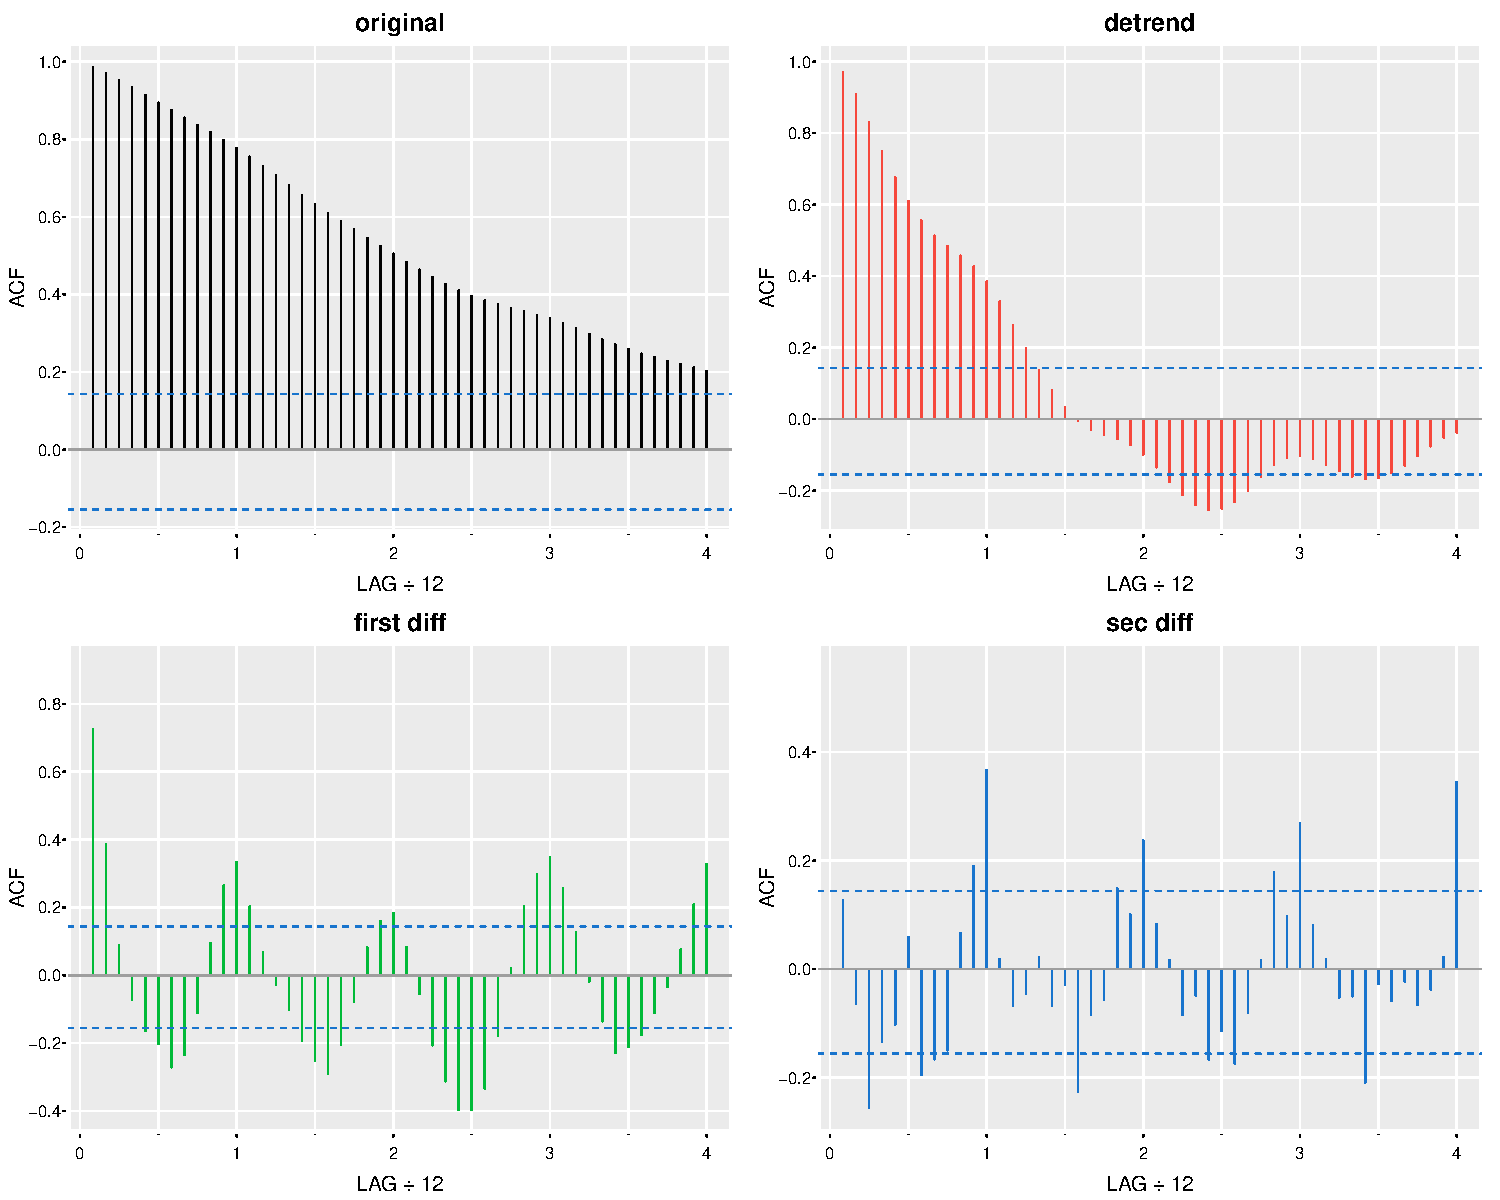
\includegraphics[width=.75\textwidth]{figure41.pdf}
\caption{ACF for detrended and differenced time series}
\label{fig:figure41}
\end{figure}

\begin{tcolorbox}[colback=code]
\subsubsection*{Hands-On Exercises} 
\begin{enumerate}
  \item Extend the mortality, temperature and pollution/particulate model by adding another component to the regression that accounts to the particulate four weeks prior; that is, add the lagged pressure $P_{t-4}$ to the regression.
  \item Draw a scatterplot matrix of of mortality $M_t$, temperate $T_t$, pressure $P_t$ and lagged pressure $P_{t-4}$, then calculate the pairwise correlations between them. Compare the relationship between $M_t$ and $P_t$ versus $M_t$ and $P_{t-4}$
\end{enumerate}

{\footnotesize \vspace{\baselineskip} Source: Shumway \& Stoffer, Chapter 2}
\end{tcolorbox}

\begin{tcolorbox}[colback=code]
\subsubsection*{Hands-On Exercises} 
\begin{enumerate}
  \item Detrend the \texttt{soi} time series data by fitting a regression of $S_t$ on time $t$. Is there a significant trend in the surface pressure?
  \item Use two different smoothing techniques to estimate the trend in the global temperature series \texttt{gtemp\_both} in the \texttt{astsa} library.
\end{enumerate}

{\footnotesize \vspace{\baselineskip} Source: Shumway \& Stoffer, Chapter 2}
\end{tcolorbox}

\begin{tcolorbox}[colback=code]
\subsubsection*{Hands-On Exercise} 
Consider the two weekly time series \texttt{oil} and \texttt{gas} in the  \texttt{astsa} library. The oil series is in dollars per barrel, while the gas series in in cents per gallon.
\begin{enumerate}
   \item Plot the data on the same graph. Do you believe the series are stationary?
   \item Apply the transformation $y_t = \nabla \log x_t$ to the data for both series
   \item Plot the transformed series on the same graph, and calculate the ACFs for both series
   \item Plot the CCF of the transformed series and comment.
\end{enumerate}

{\footnotesize \vspace{\baselineskip} Source: Shumway \& Stoffer, Chapter 2}
\end{tcolorbox}

\section{ARIMA Models}

ARIMA models, which stands for Autoregressive Integrated Moving Average, are a type of statistical models for analyzing and forecasting time series data. ARIMA is particularly suited to time series data that show non-stationarities, such as trends and seasonal patterns, and it has become a standard tool in econometrics, finance, and other fields.

ARIMA models can be divided into the following model classes:
\begin{itemize}
  \item \textbf{AR}: pure AutoRegressive models
  \item \textbf{MA}: pure Moving average models
  \item \textbf{ARMA}: model with AutoRegressive and Moving-Average terms
  \item \textbf{ARIMA}: AutoRegressive Integrated Moving-Average models (involves differencing for non-stationary time series with trend)
\end{itemize}

To simplify working with ARIMA models, the difference operator $\nabla$ is defined as:

\begin{align*}\nabla x_t = x_t - x_{t-1}\end{align*}

\noindent Building on this definition, the \emph{Backshift operator} or \emph{Lag Operator} $\operatorname{B}$ is defined as:

\begin{align*}\operatorname{B} x_t &= x_{t-1} \\
\operatorname{B}^k x_t &= x_{t-k} \\
\nabla x_t &= (1-\operatorname{B})x_t \\
\nabla^2 x_t &= (1-\operatorname{B})^2 x_t \\
 &= (1-2 \operatorname{B} + \operatorname{B}^2)x_t \\
 &= x_t - 2x_{t-1} + x_{t-2} \\
\nabla^d &= (1-\operatorname{B})^d
\end{align*}

An \emph{autoregressive model} of order $p$, denoted by AR(p), models the current value of a time series as a linear combination of previous values. The number of lagged observations used in the model is denoted by the order $p$. The AR model captures the regression of the time series on its previous values, which indicates persistence, or memory, within the series. It is defined as:

\begin{align*}
x_t = \phi_1 x_{t-1} + \phi_2 x_{t-2} + \cdots + \phi_p x_{t-p} + w_t
\end{align*}

\noindent where $w_t$ is white noise and the $\phi_i$ are model parameters\footnote{In contrast to an ''ordinary'' regression model, the $x_i$ are random effects, not fixed, because each $x_i$ has an associated error term $w_t$. This means that AR or ARIMA models in general are not estimated using OLS because the OLS assumptions are not met. Instead, AR and ARIMA models are estimated using maximum-likelihood or other methods.}.

The \emph{autoregressive operator} $\phi (B)$ is defined using the backshift operator as: 
\begin{align*}
\phi (B) &= 1 - \phi_1 B - \phi_2 B^2 - \cdots - \phi_p B^p \\
         &= \left(1 - \sum_{j=1}^p \phi_j B^j \right)
\intertext{so that the AR(p) model becomes:}
\phi (B) x_t &= w_t
\end{align*}

The theoretical ACF of a given AR(p) model can be calculated analytically. In R, the \texttt{ARMAacf()} function can be used for this by spacifying the autoregressive coefficients $\phi$. The following R code block simulates 200 observations of an AR(2) time series and plots the simulated (blue) versus theoretical (red) ACF values, shown in Figure~\ref{fig:figure18}. The theoretical values can be used to determine whether a specific time series conforms to a particular AR(p) model. The ACF of an AR(p) model is characterized by a slow decline of its values past a lag of $p$, as shown in Figure~\ref{fig:figure18}.

\begin{samepage}
\begin{Rcode}
# Theoretical ACF of an AR(2) model
ARMAacf(ar=c(1.5, -.75), lag.max=10)
# Simulate an ARIMA(2,0,0) model with those AR coefficients
t.ar = arima.sim(list(ar=c(1.5, -.75)), n=200)
# Compute and plot the ACF of the simulated series
acf1(t.ar, max.lag=25, gg=T, lwd=2, col=4)
# Add the theoretical values for comparison
lines(ARMAacf(ar=c(1.5, -.75), lag.max=26)[-1], lwd=2, col=2)
\end{Rcode}
\end{samepage}

\begin{figure}
\centering
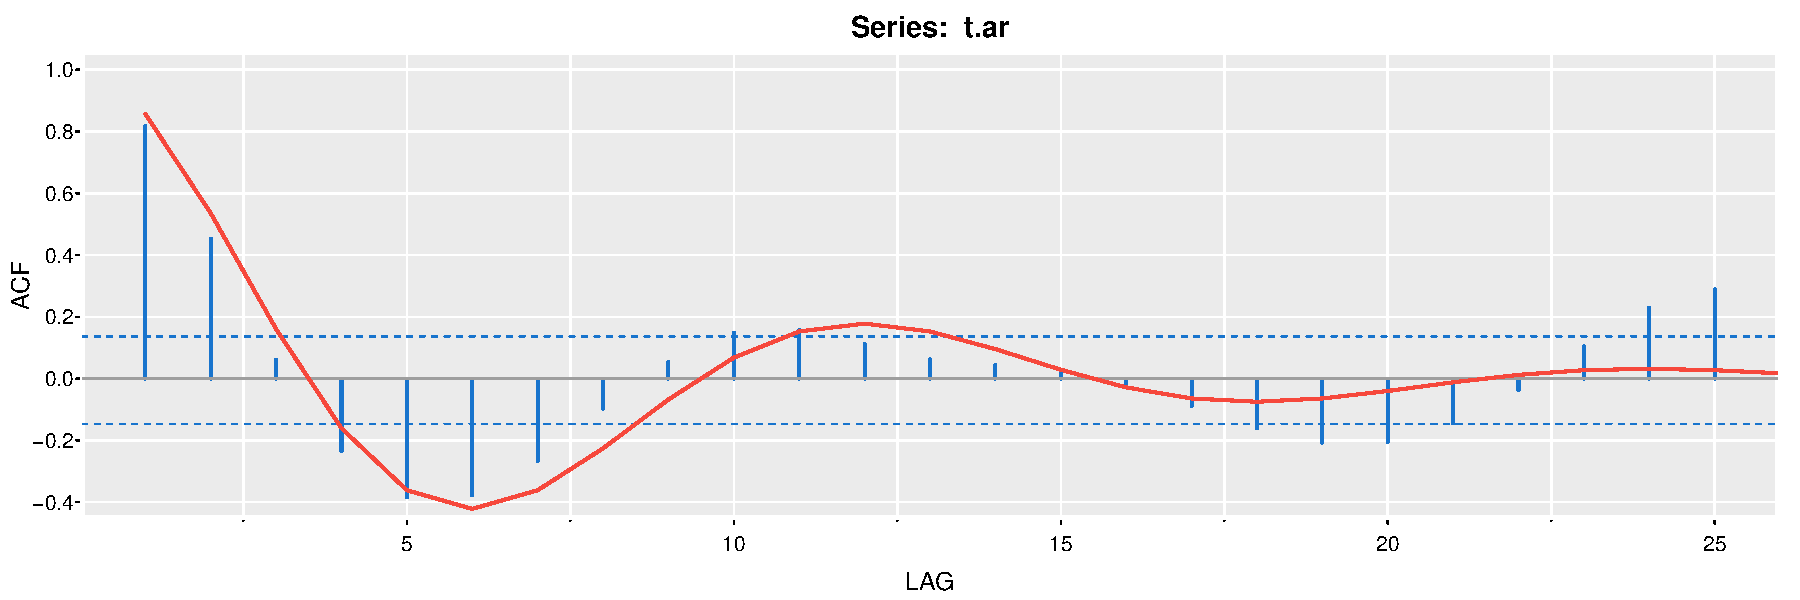
\includegraphics[width=.75\textwidth]{figure18.pdf}
\caption{Simulated (blue) and theoretical (red) ACF of an AR(2) model}
\label{fig:figure18}
\end{figure}

A \emph{moving average model} or order $q$, denoted by MA(q), models the current value of the series as a linear combination of past forecast errors, which are computed as differences between past values and their respective forecasts. The parameter $q$ specifies the number of lagged forecast errors in the prediction equation. The MA model is usefule for capturing ''shock errors'' in the model, providing a way to allow the model to adapt to sudden changes in the series. It is defined as: 

\begin{align*}
x_t = w_t + \theta_1 w_{t-1} + \theta_2 w_{t-2} + \cdots + \theta_q w_{t-q}
\end{align*}

\noindent where $w_t$ are Gaussian errors and $\theta_i$ are model parameters. \\

The \emph{moving average operator} $\theta (B)$ is defined using the backshift operator as:
\begin{align*}
\theta (B) &= 1 + \theta_1 B + \theta_2 B^2 + \cdots + \theta_q B^q \\
           &= \left(1 + \sum_{j=1}^q \theta_i B^i \right) 
\intertext{so that the MA(q) model becomes:} 
x_t &= \theta(B) w_t 
\end{align*}

%\begin{frame}{MA(1) Models}

%The MA(1) model has an ACF:
%\begin{align*}
%\rho(h) = \begin{cases}\frac{\phi}{1+\phi^2} &\quad h=1 \\ 0 &\quad h > 1 \end{cases}
%\end{align*}
%\end{frame}

The theoretical ACF of a given MA(q) model can be calculated analytically. In R, the \texttt{ARMAacf()} function can be used for this, by specifying the moving average coefficients $\theta$. Similar to the previous example, the following R code simulates 200 observations of an MA(2) model and plots the simulated (blue) versus theoretical (red) ACF values, shown in Figure~\ref{fig:figure19}. In contrast to an AR(2) model, the ACF does not gradually diminish, but becomes 0 after lag $q$. The simulated values in Figure~\ref{fig:figure19} confirm this as they are largely stastistically non-significant past a lag of 2.

\begin{samepage}
\begin{Rcode}
# Theoretical ACF of an MA(2) model
ARMAacf(ma=c(1.5, -.75), lag.max=10)
# Simulate an ARIMA(0,0,2) model with those MA coefficients
t.ma = arima.sim(list(ma=c(1.5, -.75)), n=200)
# Compute and plot the ACF of the simulated series
acf1(t.ma, gg=T, lwd=2, col=4)
# Add the theoretical values for comparison
lines(ARMAacf(ma=c(1.5, -.75), lag.max=26)[-1], lwd=2, col=2)
\end{Rcode}
\end{samepage}

\begin{figure}
\centering
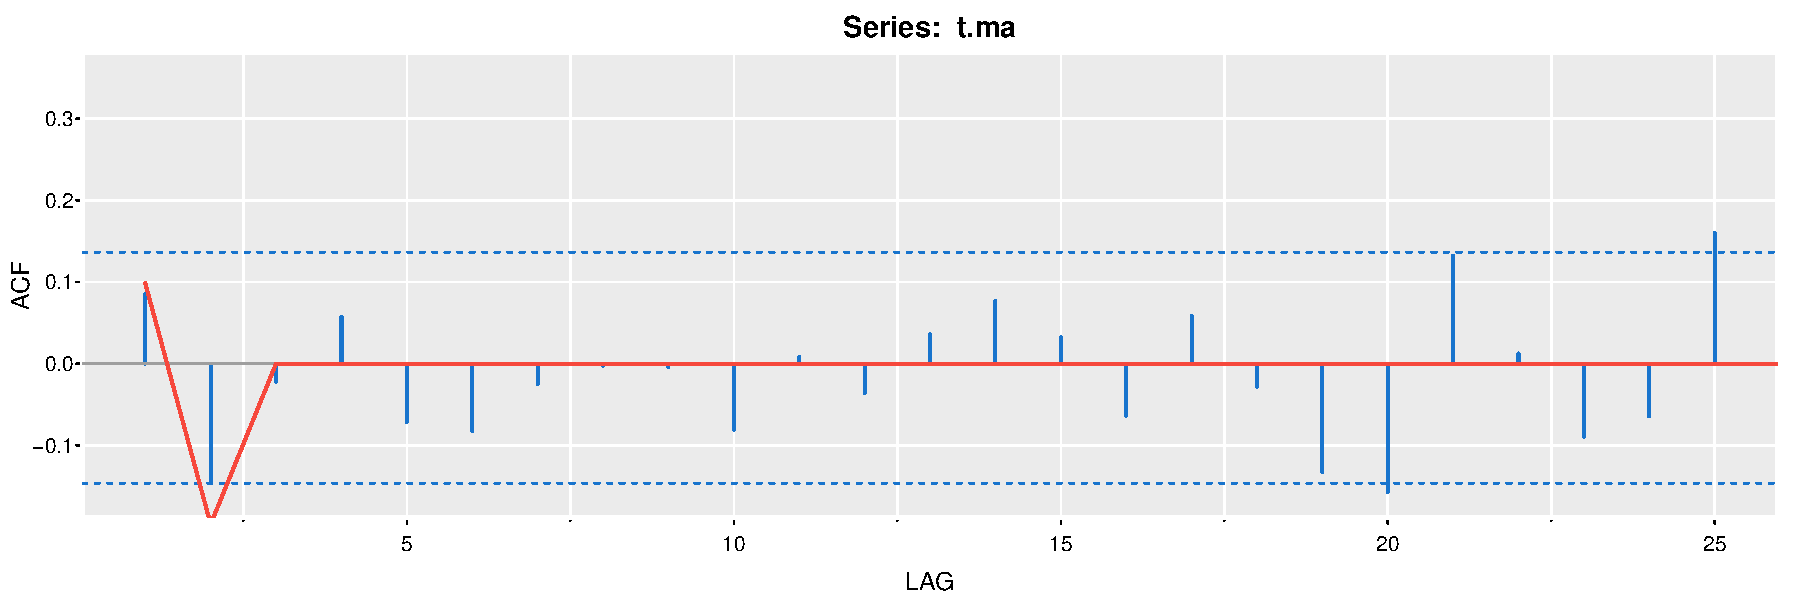
\includegraphics[width=.75\textwidth]{figure19.pdf}
\caption{Simulated (blue) and theoretical (red) ACF of an MA(2) model}
\label{fig:figure19}
\end{figure}

An \emph{autoregressive moving-average model} of order $(p, q)$, denoted by \emph{ARMA(p,q)}, combines both autoregressive and moving-average terms in the same model:

\begin{align*}
x_t &= \alpha + \phi_1 x_{t-1} + \cdots + \phi_p x_{t-p} + w_t + \theta_1 w_{t-1} + \cdots + \theta_q w_{t-q} 
\end{align*}
\noindent Using the AR and MA operators defined above, this model can be written as:
\begin{align*}
\phi(B) x_t &= \theta (B) w_t 
\end{align*}

It turns out that every ARMA model has an equivalent MA only model. However, this equivalent MA model in theory has an inifinite number of MA terms. In practice, a reasonable approximation can be achieved by retaining a limited number of MA terms.

Moreover, many ARMA models (the class of invertible ones) have an equivalent AR models. Again, this equivalent model has an infinite number of AR terms and again, in practice, reasonable approximations can be achieved by retaining a limited number of AR terms.

Equivalent models can be found using the \texttt{ARMAtoMA()} and \texttt{ARMAtoAR()} functions in the \texttt{astsa} library, which return the MA and AR coefficients of the equivalent models, as shows in the following R code example:

\begin{samepage}
\begin{Rcode}
library(astsa)
# MA coefficients of equivalent MA models
ARMAtoMA(ar = c(1.5, -.75), lag.max=10)
ARMAtoMA(ar = c(-.5), ma = c(-.9), lag.max=10)
# AR coefficients of equivalent AR models
ARMAtoAR(ma = c(1.5, -.75), lag.max=10)
ARMAtoAR(ar = c(-.5), ma = c(-.9), lag.max=10)
\end{Rcode}
\end{samepage}

As shown in Figures~\ref{fig:figure18} and \ref{fig:figure19}, the ACF of AR and MA models behave differently. Similarly, the PACF behaves differently for the two types of models. Figure~\ref{fig:figure20} shows the ACF and the PACF for an AR(2) model. While the ACF diminishes gradually, the PACF is zero immediately after lag $2$. These properties of the ACF and PACF can be used to select a suitable statistical model to fit a given time series, as shown in Table~\ref{tab:modelselection}. When a AR gradually diminishes and the PACF cuts off suddenly after a lag $p$, this is an indication that an AR(p) model is suitable. Conversely, when the ACF cuts off suddenly after lag $q$ and the PACF diminishes gradually, this is an indication for an MA(q) model. When neither ACF nor PACF cut off suddenly, a mixed ARMA(p, q) model should be fitted.


\begin{figure}
\centering
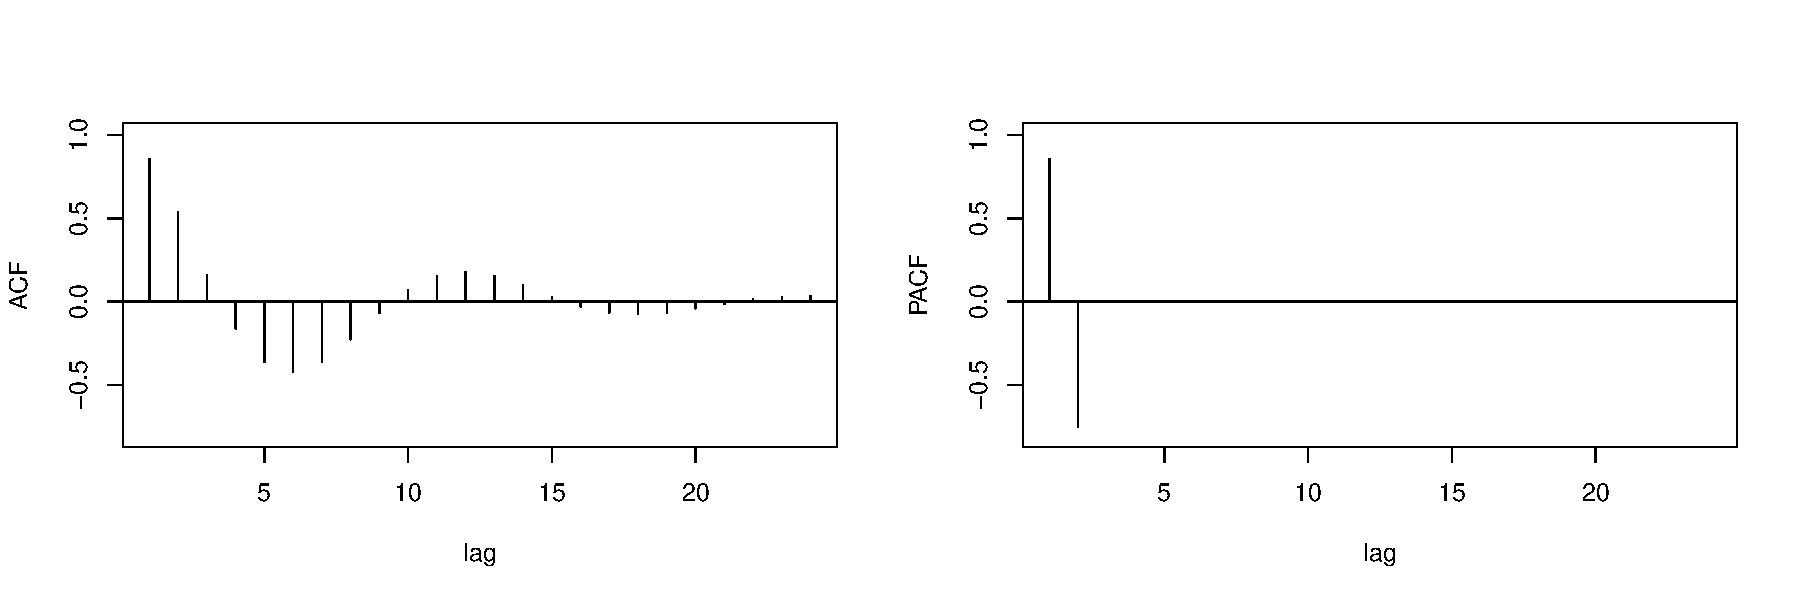
\includegraphics[width=.9\textwidth]{figure20.pdf}
\caption{ACF and PACF of an AR(2) model}
\label{fig:figure20}
\end{figure}


\begin{table}
\centering
\renewcommand{\arraystretch}{1.5}
\begin{tabular}{r|c|c|c} \hline
 & AR(p) & MA(q) & ARMA (p, q) \\ \hline
 ACF & Tails off & Cuts off after laq $q$ & Tails off \\
 PACF & Cuts off after lag $p$ & Tails off & Tails off \\ \hline
\end{tabular} \\

\vspace{\baselineskip}
\scriptsize Source: Shumway\&Stoffer, Table 3.1 \normalsize
\caption{Properties of the ACF and PACF for AR and MA models}
\label{tab:modelselection}
\end{table}

A full \emph{autoregressive integrated moving average} ARIMA(p, d, q) model adds a differencing term to the ARMA(p,q) model to achieve weak stationarity of the time series. The AR operator can be factorized by $(1-B)$, so that:
\begin{align*}
\phi (B) &= \left(1 - \sum_{j=1}^{p'} \phi_j B^j \right) \\
&= \left(1 - \sum_{j=1}^{p'-d} \phi_j B^j \right) (1 - B)^d 
\end{align*}
\noindent With $p=p'-d$, the ARIMA(p,d,q) model is then:
\begin{align*}
\left( 1 - \sum_{j=1}^p \phi_j B^j \right) (1-B)^d x_t &= \left( 1 + \sum_{j=1}^q \theta_j B^j \right) w_t
\intertext{This can be generalized to:}
\left( 1 - \sum_{j=1}^p \phi_j B^j \right) (1-B)^d x_t &= \delta + \left( 1 + \sum_{j=1}^q \theta_j B^j \right) w_t
\end{align*} 

\section{Fitting an ARIMA Model}

Fitting an ARIMA model to time series data involves the following steps, from initial data analysis and transformation to final model selection:

\begin{enumerate}
  \item Plot the data
  \item Possibly transform the data
  \item Assess stationarity
  \item Possibly difference the data
  \item Identify the dependence orders (p, q) of the model
  \item Estimate parameters
  \item Model diagnostics
  \item Model selection
\end{enumerate}

Plotting the data is useful as an initial visual assessment of stationarity, trends, or seasonality. A number of transformations have been discussed earlier that may be useful to ''stabilize'' a time series. If the series after transformation is still not stationary, differencing can remove trends and seasonal components. Determining the order of differencing needed to achieve stationarity is often done by trial and error, reassessing stationarity after each difference. A slow decay in the sample ACF $\hat\rho(h)$ typically indicates a need for differencing. However, over-differencing can introduce dependence where non actually exists. Typically, differencing should be done in small steps, beginning with a first difference, and then repeatedly checked with the ACF.

Identifying the initial ARMA order $p$ and $q$ should be done based on the ACF and PACF functions, using Table~\ref{tab:modelselection} as a basis. Often, multiple model may need to be tried, altering the AR and MA orders $p$ and $q$ in small steps. 

The following R code example uses a quarterly time series of the US gross national product (\texttt{gnp}) from the \texttt{astsa} library as an example. The \texttt{acf2()} function of the \texttt{astsa} library produces simultaneous plots of ACF and PACF for ease-of-use. The time series is then log-transformed and differenced once. The results are shown in Figure~\ref{fig:figure22}.

\begin{samepage}
\begin{Rcode}
# Plot data
plot(gnp)
# Plot ACF
acf2(gnp, 50)
# Log transform, and first order differencing
gnpgr = diff(log(gnp))
# Plot transformed and differenced data
plot(gnpgr)
# Plot ACF of transformed and differenced data
acf2(gnpgr, 24)
\end{Rcode}
\end{samepage}

\begin{figure}
\centering
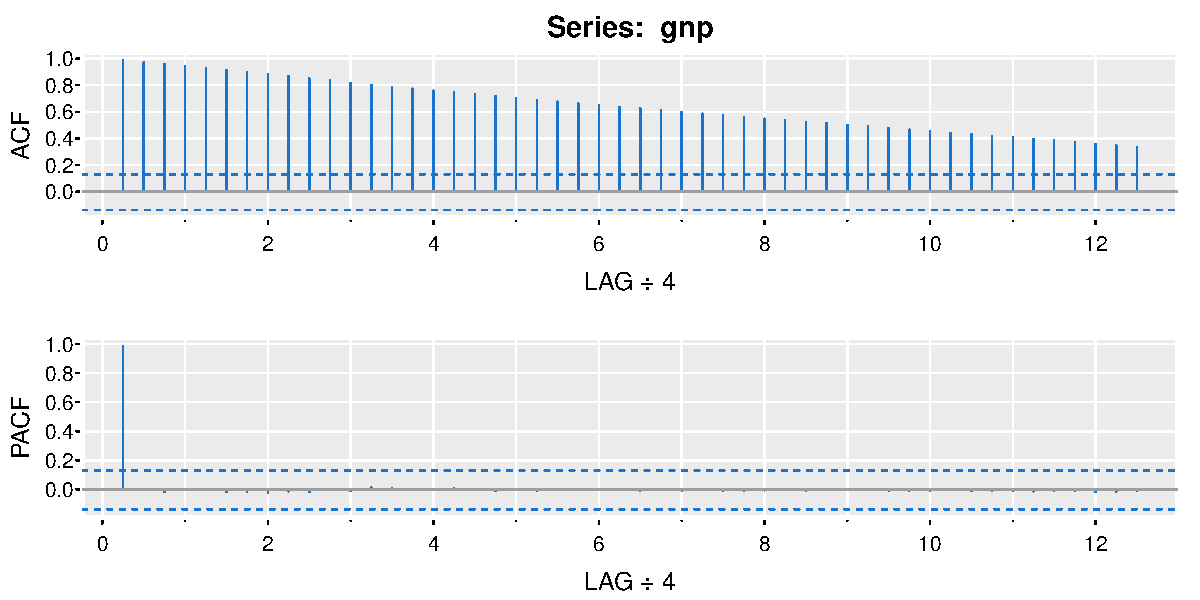
\includegraphics[width=.75\textwidth]{figure22.pdf} \\
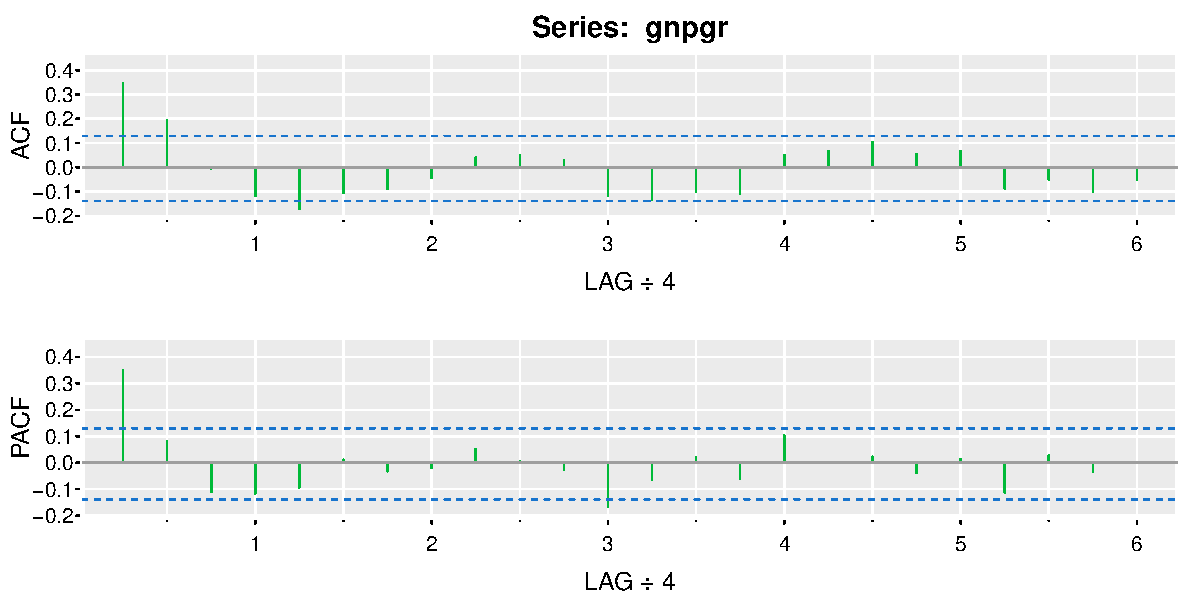
\includegraphics[width=.75\textwidth]{figure23.pdf}
\caption[ACF and PACF after transformations]{ACF and PACF of the original time series (top) and of the log-transformed and differenced series (bottom)}
\label{fig:figure22}
\end{figure}

Note how the ACF of the original series diminishes very gradually, indicating the need for differencing. The sample ACF of the transformed and differenced series shows a gradual decline after a lag of $2$, while the sample PACF of the transformed and differenced series cuts off to non-significance after a lag of $1$. Together, this indicates that the time series may be appropriately modeled using an AR(1) model or an MA(2) model. Converting the AR(1) model to an equivalent MA model shows that the two initial models are approximately equivalent. Note that the following R code block uses the \texttt{sarima()} function from the \texttt{astsa} library because this function also produces the diagnostic plots shown in Figures~\ref{fig:figure24} and \ref{fig:figure25}. This function can fit ARIMA models, as in the following example, but can also fit seasonal ARIMA, or SARIMA, models.

\begin{samepage}
\begin{Rcode}
# Fit an AR(1) model
sarima(gnpgr, 1, 0, 0)
# Fit an MA(2) model
sarima(gnpgr, 0, 0, 2)
# Models are roughly equivalent
ARMAtoMA(ar=0.35, ma=0, 10)
\end{Rcode}
\end{samepage}

\begin{figure}
\centering
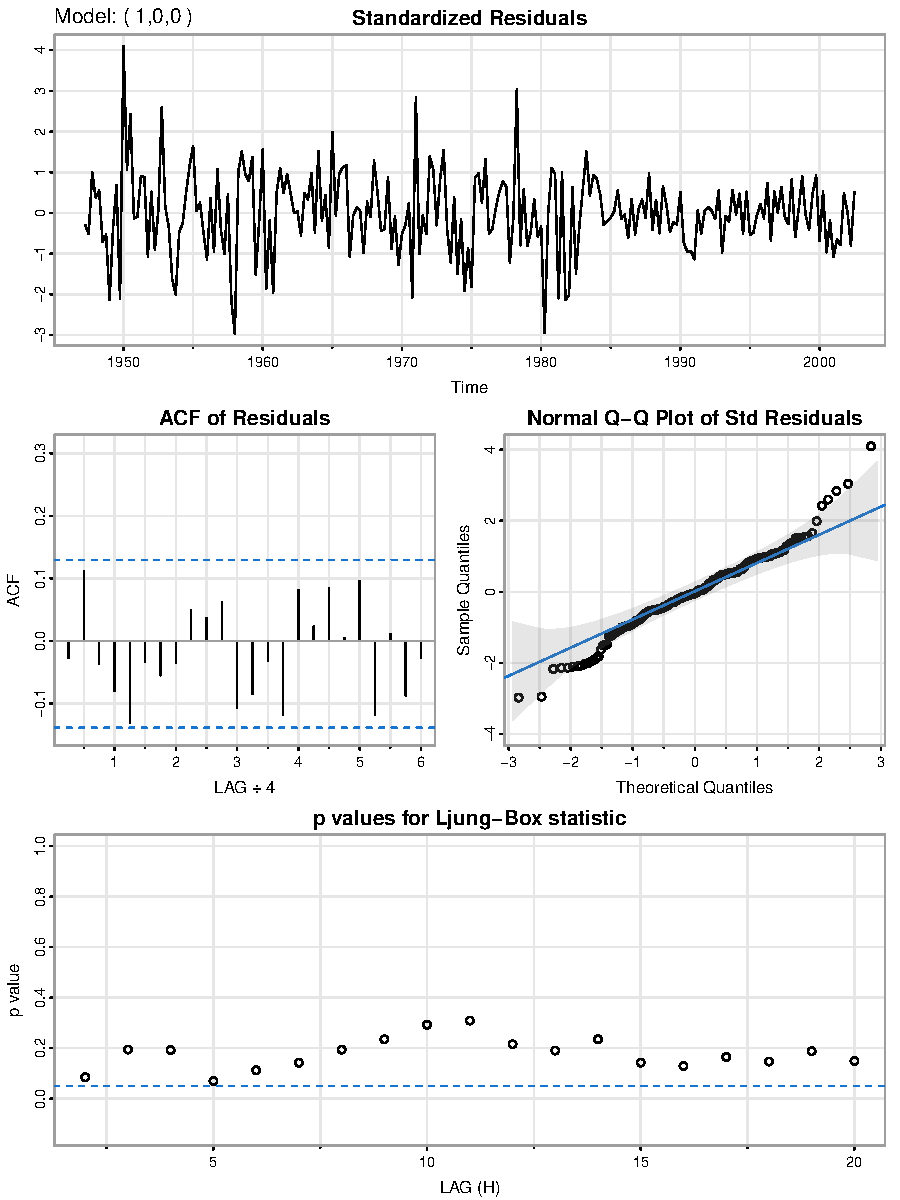
\includegraphics[width=.75\textwidth]{figure24.pdf}
\caption{Diagnostics for an AR(1) model fitted to the GNP time series}
\label{fig:figure24}
\end{figure}

\begin{figure}
\centering
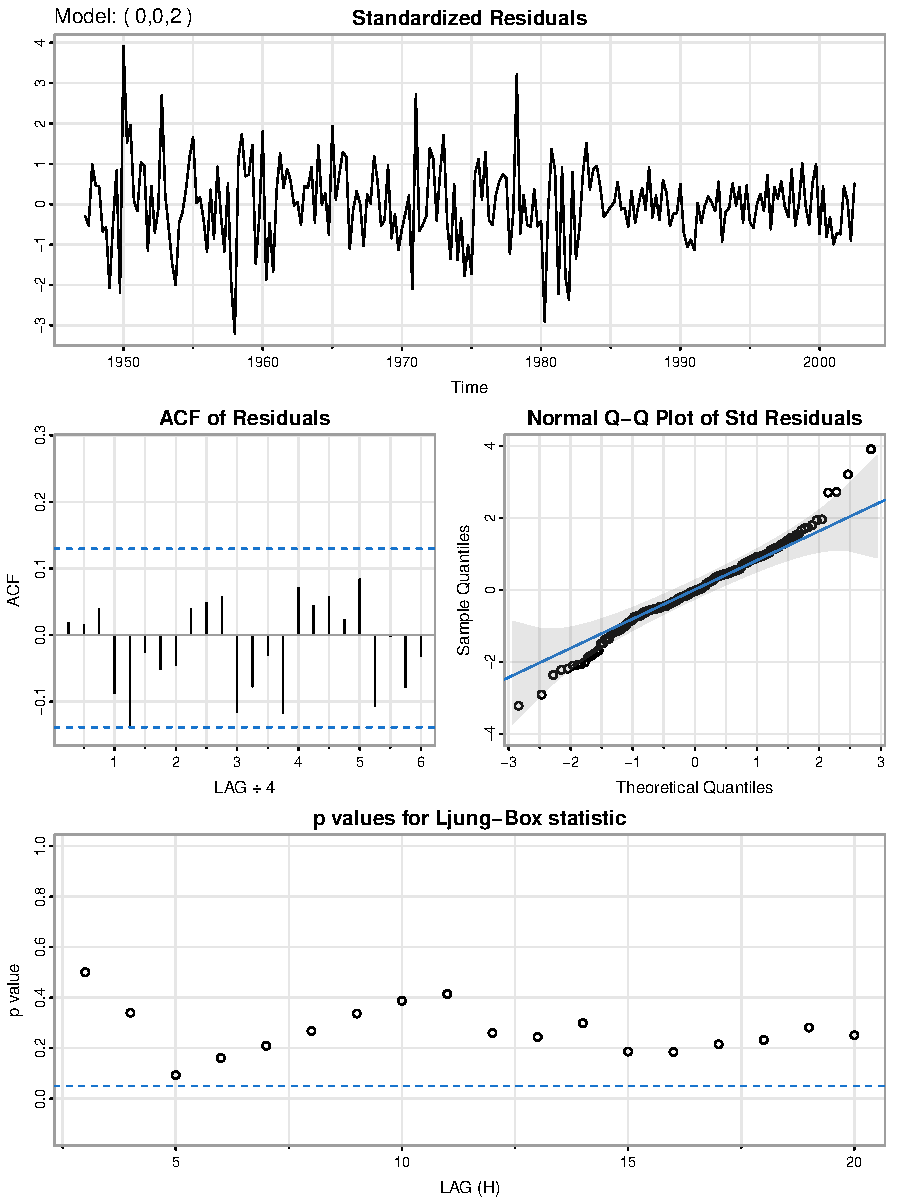
\includegraphics[width=.75\textwidth]{figure25.pdf}
\caption{Diagnostics for an MA(2) model fitted to the GNP time series}
\label{fig:figure25}
\end{figure}

ARIMA model diagnostics focus on the residuals of the fitted model and typically assess the following criteria:

\begin{itemize}
   \item Standardized residuals should be Gaussian ($\mu=0$, $sd=1$)
   \item Residuals should not be autocorrelated
   \item Residual ACF should be Gaussian with $\mu=0$ and $sd=1/\sqrt{n}$
   \item Ljung-Box statistic $Q$ of the error ACF $\hat\rho_e$ for different maximum lags $H$ should be larger than the $1-\alpha$ quantile of the $\chi^2_{H-p-q}$ distribution (i.e. the test statistic is not statistically signifantly different from $0$)
   \begin{align*}
   Q = n(n+2) \sum_{h=1}^H \frac{\hat\rho_e^2(h)}{n-h}
   \end{align*}
\end{itemize}

The diagnostic plots in Figure~\ref{fig:figure24} and \ref{fig:figure25} shows the residuals in the top panels. There are no visible trends or regularities and a few large outliers, but these can be expected from a Gaussian distribution. The ACF of the residuals in the middle left panel show that they are not autocorrelated and the QQ plot of residuals shows some deviations from a linear diagonal in the bottom and top portions, indicating that the model over- and under-estimates extreme values. The bottom panel in each figure shows the probability values (p-values) for the Ljung Box statistics and the $1-\alpha$ dashed horizontal line. For both models, the p-values of the Ljung Box statistic are above the horizontal line, that is, they are not significantly different. In summary, both models show good fit to the data.

Because fitting a model typically uses maximum-likelihood estimation (MLE), the model choice is often based on information criteria that are based on the log-likelihood $L$ of the model. Because more complex models naturally achieve a better fit to the training data, that is, they have a smaller bias, the log-likelihood is adjusted (penalized) for model complexity, that is, the number of parameters $k$, and is also adjusted for sample size $n$. All information-theoretic criteria express a \emph{relative} quality of fit with \emph{smaller values being better}. There are no absolute cut-off values that would indicate a well-fitting model.

\begin{align*}
\operatorname{AIC} &= -2 \log L + 2k  \qquad \text{\footnotesize Akaike Information Criterion}\\
\operatorname{AICc} &= AIC + \frac{2k(k+1)}{n-k-1} \qquad \text{\footnotesize Akaike Information Criterion, corrected}\\
\operatorname{BIC} &= -2 \log L + k \log n \qquad \text{\footnotesize Bayesian Information Criterion}
\end{align*}

\noindent The R output of the \texttt{sarima()} function shows very similar model fit values:

\begin{samepage}
\begin{textcode}
> sarima(gnpgr, 1, 0, 0)

AIC = -6.44694  AICc = -6.446693  BIC = -6.400958 
\end{textcode}
\end{samepage}

\begin{samepage}
\begin{textcode}
> sarima(gnpgr, 0, 0, 2)

AIC = -6.450133  AICc = -6.449637  BIC = -6.388823 
\end{textcode}
\end{samepage}

Once the analyst has selected the final model and is satisfied that it fits well, future values of the time series can be forecasted from the fitted model. An important property of ARIMA predictions is that they quickly settle to the mean, with a constant prediction error, reflecting the stationarity of the differenced and transformed time series.

The following R code example shows forecasting from using the \texttt{sarima.for()} function in the \texttt{astsa} library. The results are shown visually in Figure~\ref{fig:figure21}, where the prediction error is indicated by the gray shading.

\begin{Rcode}
forecasts <- sarima.for(gnpgr, n.ahead=10, p=1,d=0,q=0)
\end{Rcode}

\begin{figure}
\centering
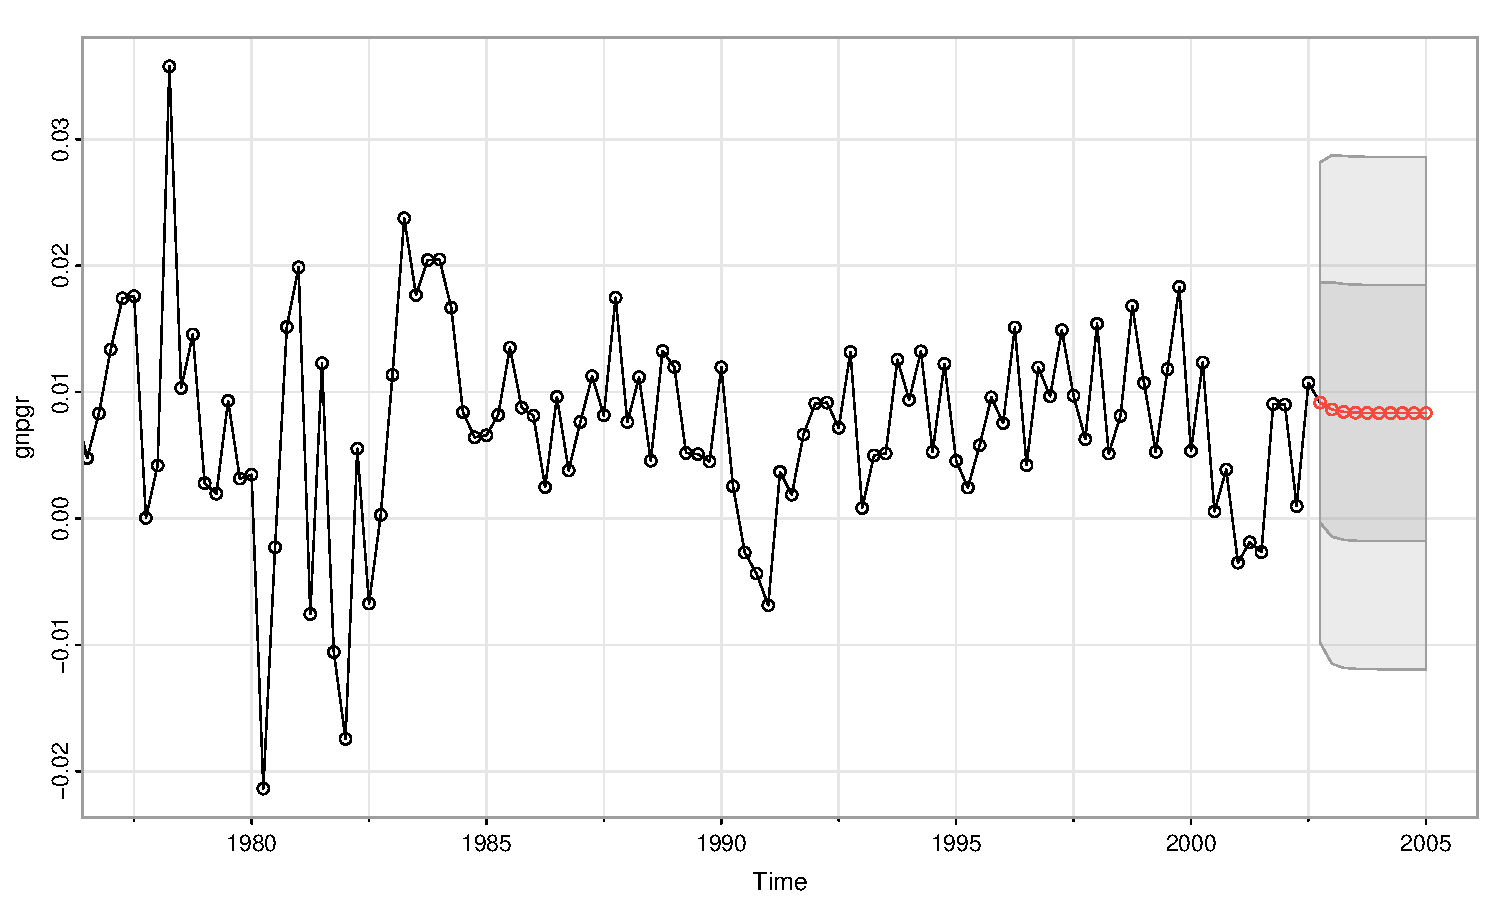
\includegraphics[width=.75\textwidth]{figure21.pdf}
\caption[Forecasting from an ARIMA(1,0,0) model]{Forecasting from an ARIMA(1,0,0) model with estimated prediction errors}
\label{fig:figure21}
\end{figure}

\section{GARCH Models}

General Autoregressive Conditional Heteroscedasticity (GARCH) models are a family of time series models that are used to estimate the volatility and conditional variance of time series data, particularly of financial time series that exhibit time-varying volatility and volatility clustering. GARCH models are fundamental in the field of financial econometrics for modeling financial time series data.

GARCH models predict the current variance (that is, the volatility or variability, not the actual values) as a function of past squared ''innovations'' (which represent unexpected shocks or news in the data) and past conditional variances. In other words, the variance at any time depends on the information available up to the previous period. GARCH models are particularly effective at modeling volatility clustering, a phenomenon common in financial time series where high-volatility events tend to cluster together.

GARCH models are extensively used in risk management, asset pricing, and financial forecasting. They help in estimating the volatility of asset returns for pricing derivatives, calculating the value at risk for risk management, or forecasting volatility for portfolio optimization. 

An ARCH model considers a series of ''returns'', which are defined as deviations from the prior value:

\begin{align*}
r_t = \frac{x_t - x_{t-1}}{x_{t-1}} \qquad \text{(''Return'')}
\end{align*}

The series of returns is modelled as the product of a stochastic component $\epsilon_t$ and a time-dependent standard deviation $\sigma_t$

\begin{align*}
r_t &= \sigma_t \epsilon_t
\end{align*}

The ARCH model considers the time-dependent variance $\sigma_t^2$ at time $t$ as a function of the previous returns. For example, in the ARCH(1) model the variance $\sigma_t^2$ at time $t$ depends on the immediately prior squared return:

\begin{align*}
\sigma_t^2 &= \alpha_0 + \alpha_1 r_{t-1}^2
\end{align*}
\noindent where $\epsilon_t$ is Gaussian.

\begin{samepage}
The general ARCH(q) model of order q is defined as follows. Again, the variance depends on the prior squared returns:
\begin{align*}
\sigma_t^2 &= \alpha_0 + \alpha_1 r_{t-1}^2 + \alpha_2 r_{t-2}^2 + \ldots + \alpha_q r_{t-q}^2 \\
           &= \alpha_0 + \sum_{i=1}^q \alpha_i r_{t-i}^2
\end{align*}
\end{samepage}

ARCH models can be combined with ARIMA models so that the ARCH model describes the error term. A simple example is an AR(1) model with ARCH(1) error terms:
\begin{align*}
x_t = \phi_0 + \phi_1 x_{t-1} + \sigma_t \epsilon_t \quad \text{where} \quad \sigma_t = \alpha_0 + \alpha_1 x_{t-1}^2
\end{align*} 

As an example, consider the US gross national product quarterly time series from the \texttt{astsa} library. An initial AR(1) model shows that the squared residuals have some dependence. This dependence can be accounted for by explicitly modeling the residuals as ARCH(1). The \texttt{fGarch} library for R provides the \texttt{garchFit()} function to these kinds of models. The squared residuals of the final model are shown in Figure~\ref{fig:figure35}.

\begin{figure}
\centering
\centering
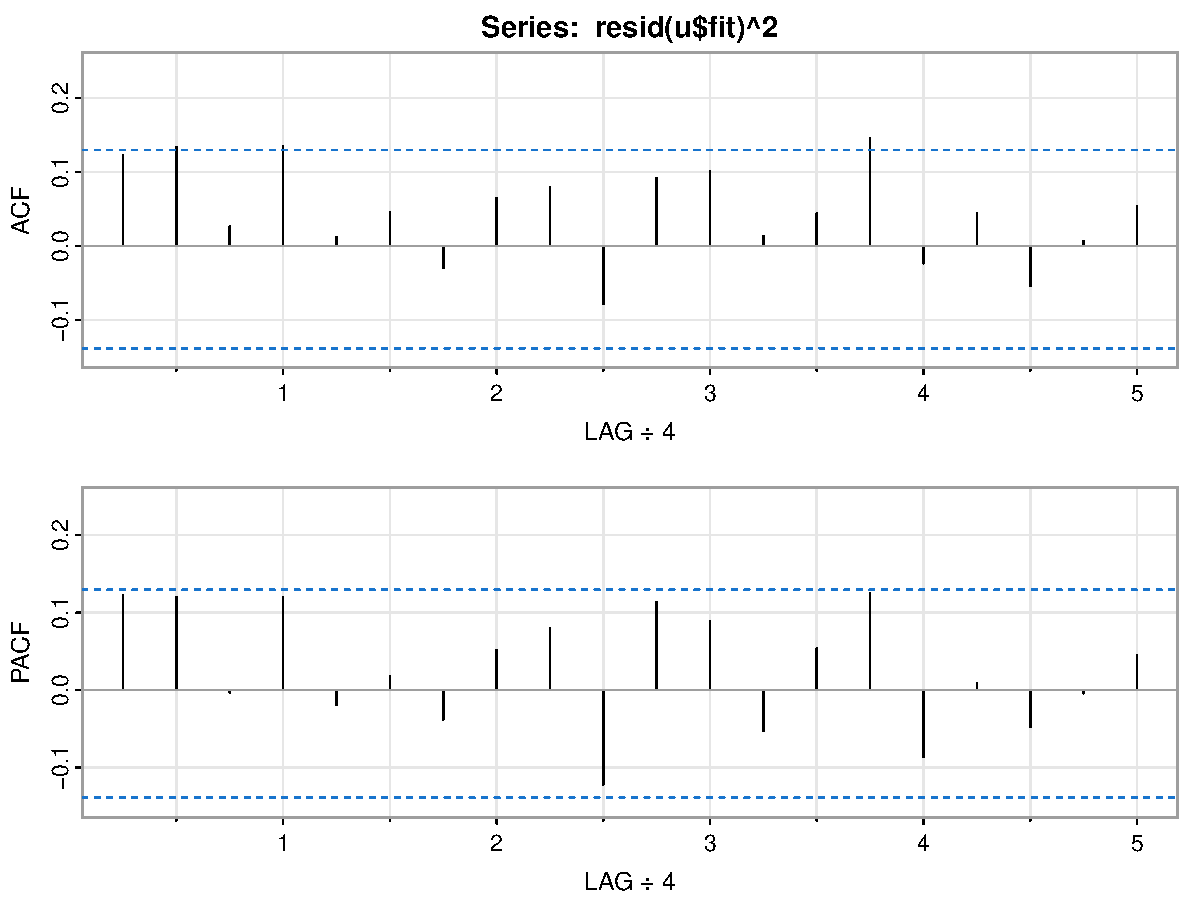
\includegraphics[width=.75\textwidth]{figure35.pdf}
\caption[Squared residuals after fitting an AR(1)+ARCH(1) model]{Squared residuals after fitting an AR(1)+ARCH(1) model to the US GNP time series data}
\label{fig:figure35}
\end{figure}

\begin{samepage}
\begin{Rcode}
library(astsa)
# Fit an AR(1) model to the differenced, log-transformed series
u = sarima(diff(log(gnp)), 1, 0, 0)
# Examine the squared residuals
acf2(resid(u$fit)^2, 20)

library(fGarch)
# Fit an AR(1) + ARCH(1) model to the differenced, log-transformed 
# series and show the summary
summary(garchFit(~arma(1,0)+garch(1,0), diff(log(gnp))))
\end{Rcode}
\end{samepage}

An extension to ARCH is to model the variance not only as a function of previous returns, but also as a function of the $p$ prior variances. In other words, the variance is modelled as an autoregressive model in addition to the ARCH(q) terms. This leads to a Generalized ARCH model, that is, a GARCH(p, q) model:

\begin{align*}
\sigma_t^2 &= \omega + \alpha_1 r_{t-1}^2 + \cdots + \alpha_q r_{t-q}^2 \\
           & \qquad \qquad + \beta_1 \sigma_{t-1}^2 + \cdots + \beta_p \sigma_{t-p}^2 \\
           &= \omega + \sum_{j=1}^q \alpha_j r_{t-j}^2 + \sum_{j=1}^p \beta_j \sigma_{t-j}^2
\end{align*}

The following R example models the Dow Jones Industrial Average stock market time series values (data set \texttt{djiar} in library \texttt{astsa}) using an AR(1)+GARCH(1,1) model. Parameter estimates are shown below. Various diagnostic plots are available using the \texttt{plot()} function for the resulting \texttt{garchFit} object and are shown in Figure~\ref{fig:figure38a}. 

\begin{samepage}
\begin{Rcode}
library(zoo)
library(fGarch)
# Log transform
djiar = diff(log(djia$Close))[-1]
# Fit an AR(1) + GARCH(1,1) model
djia.g <- garchFit(~arma(1,0)+garch(1,1), data=djiar)
# Show summary information
summary(djia.g)
# Different plots available
par(mfrow=c(5,2)
plot(djia.g, which=1:10)
\end{Rcode}
\end{samepage}

\begin{figure}
\centering
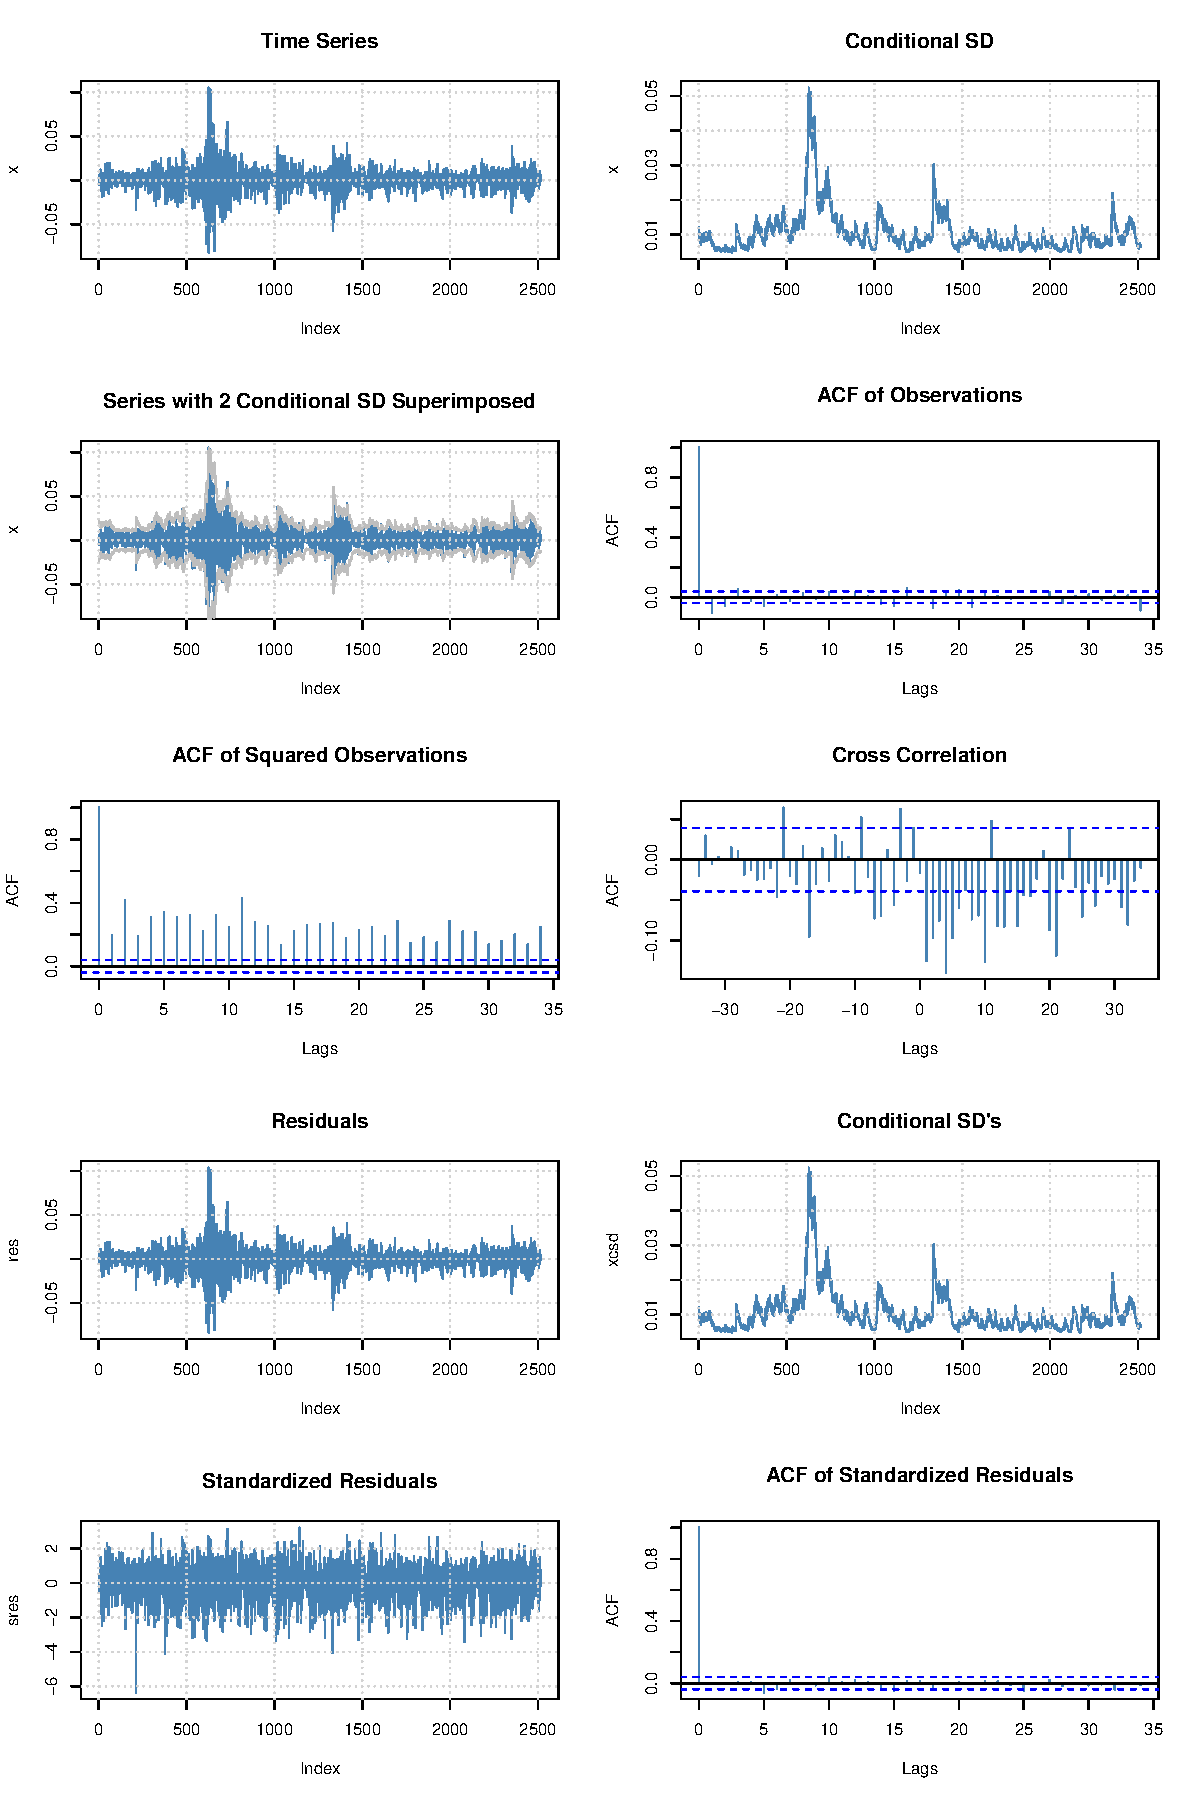
\includegraphics[width=\textwidth]{figure38a.pdf}
\caption{Diagnostic plots for a GARCH model}
\label{fig:figure38a}
\end{figure}

\begin{samepage}
\begin{textcode}
         Estimate  Std. Error  t value Pr(>|t|)    
mu      8.585e-04   1.470e-04    5.842 5.16e-09 ***
ar1    -5.532e-02   2.023e-02   -2.735 0.006238 ** 
omega   1.610e-06   4.459e-07    3.611 0.000305 ***
alpha1  1.244e-01   1.660e-02    7.496 6.55e-14 ***
beta1   8.700e-01   1.526e-02   57.022  < 2e-16 ***
shape   5.979e+00   7.917e-01    7.551 4.31e-14 ***
---
Log Likelihood:
 8249.619    normalized:  3.27756 
\end{textcode}
\end{samepage}

\section*{Appendix -- Basic Time Series Functions in R}

\renewcommand{\arraystretch}{1.25}
\begin{tabularx}{\textwidth}{l|X} \hline
\multicolumn{2}{c}{\textbf{base or stats}} \\ \hline
\texttt{filter} & Filters time series, through moving averages or autoregression \\
\texttt{lag} & Creates a lagged version of a time series by shifting the timebase back \\
\texttt{diff} & Creates lagged differences \\ 
\texttt{plot.ts} & Plot a time series \\
\texttt{ts.plot} & Plot multiple time series \\
\texttt{lag.plot} & Scatterplot of lagged values \\
\texttt{acf} & ACF and plot \\
\texttt{ccf} & CCF and plot \\ 
\texttt{time} & Creates the vector or times at which a time series was sampled \\
\texttt{cycle} & Gives the positions in the cycle of each observation \\
\texttt{frequency} & Number of samples per unit time \\
\texttt{ts.intersect} & Bind time series together that have a common frequency. Restrict to time covered by all series \\
\texttt{ts.union} & Bind time series together that have a common frequency. Pad with NA if necessary \\ 
\texttt{ar} & Fit an autoregressive model \\ 
\texttt{arima} & Fit an ARIMA model \\ \hline
\multicolumn{2}{c}{\textbf{astsa}} \\ \hline
\texttt{tsplot} & Plot a time series \\
\texttt{acf1} & ACF and plot \\
\texttt{ccf2} & CCF and plot \\
\texttt{sarima} & Fit seasonal ARIMA models (and nice diagnostic plots) \\
\texttt{lag1.plot} & Scatterplot of lagged values \\ \hline
\end{tabularx}

\FloatBarrier
\section{Review Questions}

\paragraph*{Introduction}
\begin{enumerate}[nosep]
    \item What is time series analysis and why is it important in various fields such as economics, finance, and natural sciences?
    \item What are some essential preprocessing steps required before performing time series analysis?
    \item Compare and contrast the time-domain approach and the frequency-domain approach in time series analysis. Which approach is particularly useful for forecasting and why?
\end{enumerate}
\paragraph*{Time Series Statistical Models}
\begin{enumerate}[nosep,resume*]
    \item Explain the Moving Average (MA) model and describe how it uses past error terms to forecast future values. What are the assumptions about these error terms?
    \item Discuss how the Moving Average (MA) model can be utilized to detect underlying patterns in a time series that exhibits random fluctuations. What limitations does this model have in handling trend and seasonality?
    \item Explain the implications of choosing different window sizes (the number of terms included) in the Moving Average model. How does it affect the forecasts and smoothing?
    \item Describe how the Autoregressive (AR) model differs from the MA model and provide an example of its application in economic or financial time series.
    \item In the context of the AR model equation $x_t = x_{t-1} - 0.9 x_{t-2} + w_t$, analyze the impact of changing the coefficient $-0.9$ to values closer to 0 or 1.
    \item What is a Random Walk with Drift? Describe how it models time series data and give an example of its application in financial markets.
    \item Critique the usefulness of the Signal in Noise model in various fields such as economics, engineering, and environmental science. How might the assumptions of this model limit its application?
    \item Critically evaluate the effectiveness of each model (MA, AR, Random Walk with Drift, Signal in Noise) in handling different types of time series data.
\end{enumerate}
\paragraph*{Smoothing a Time Series}
\begin{enumerate}[nosep,resume*]
    \item Explain the purpose of smoothing in time series analysis. What are the general goals of this technique?
    \item Describe the moving average smoothing method. How does this method use weights to smooth data, and what are the effects of changing these weights?
    \item Discuss how the moving average method helps in reducing the impact of random fluctuations in the data. What challenges might arise when using this method on time series with trends or seasonality?
    \item Explain what kernel smoothing is and how it uses a Gaussian kernel to weigh data points. How does the choice of bandwidth affect the smoothing?
    \item Detail the Lowess regression method. How does this method determine the weights for smoothing and how do these weights contribute to the robustness against outliers?
    \item Explain the role of the parameter \texttt{f} in the \texttt{lowess()} function in R. How does changing the value of \texttt{f} affect the results of the Lowess smoothing?
    \item Define smoothing splines and describe how they fit a spline function to the data. What does the regularization term in the loss function achieve?
    \item Compare and contrast the advantages and potential drawbacks of using moving average, kernel smoothing, Lowess regression, and smoothing splines. When might one method be preferred over the others based on the characteristics of the time series data?
\end{enumerate}
\paragraph*{Time Series Regression}
\begin{enumerate}[nosep,resume*]
    \item Define time series regression and explain how it differs from other types of time series analysis such as autoregressive models.
    \item Describe the significance of including time as a variable in the regression models. What does this imply about the data and its relationship over time?
    \item Discuss the use of lagged variables in time series regression. What are the benefits of including lagged terms?
\end{enumerate}
\paragraph*{Stationarity}
\begin{enumerate}[nosep,resume*]
    \item Explain the difference between strict and weak stationarity. Why is weak stationarity more commonly used in statistical analysis of time series?
    \item Elaborate on the impact of non-stationarity on the predictive performance of time series models. How does failing to account for stationarity potentially mislead forecasting?
    \item Critique the assumption of constant variance in the definition of weak stationarity. How might changes in variance over time affect the validity of time series models?
    \item Explain how the concept of weak stationarity might still inadequately describe the nature of certain financial time series. What alternative forms of stationarity might be considered?
    \item Discuss how the mean, variance, and autocovariance function must behave for a time series to be considered weakly stationary.
    \item Define autocovariance and autocorrelation. How are these metrics useful in analyzing the properties of a time series?
    \item Analyze the implications of having a high autocorrelation at large lags for a given time series. What might this indicate about the underlying data generation process?
    \item What does it indicate if the ACF values are outside the 95\% confidence interval? How does this help in determining whether a time series is white noise?
    \item Describe how you would assess the stationarity of a time series using graphical methods in R. What plots would you use and what features would you look for?
\end{enumerate}
\paragraph*{Dealing with Non-Stationarity}
\begin{enumerate}[nosep,resume*]
    \item Discuss how the Box-Cox transformation generalizes other forms of transformations like logarithmic and square root transformations. What is the significance of the parameter $\lambda$ in this transformation?
    \item Explain the statistical reasoning behind using logarithmic transformations for time series data. What types of data characteristics make this transformation particularly effective?
    \item Explain the process of detrending a time series. Why is it necessary, and how does it differ from differencing?
    \item Describe the impact of detrending and differencing on the forecasting accuracy of a time series model. How might these preprocessing steps improve or impair the model's performance?
    \item Provide a detailed explanation of the first and second differences of a time series. Under what circumstances might second differencing be necessary?
    \item Explain how the autocorrelation function (ACF) can be used to verify the effectiveness of detrending and differencing interventions on a time series.
\end{enumerate}
\paragraph*{ARIMA Models}
\begin{enumerate}[nosep,resume*]
    \item Define an ARIMA model and explain the components of its notation: ARIMA(p, d, q).
    \item Describe a moving average model of order $q$, MA(q). How does it model the current value of the series?
    \item Describe the structure of an autoregressive model of order $p$, AR(p). What does it mean for the model to have ''memory'' or ''persistence''?
    \item Discuss the role of the differencing operator $\nabla$ in making a time series stationary. How does this relate to the integrated component of an ARIMA model?
    \item Explain the purpose of the backshift or lag operator $B$ in the context of ARIMA models. Provide an example of how it is used to define the differencing of a series.
    \item Explain how the autoregressive operator $\phi(B)$ is used to form the equation of an AR(p) model.
    \item Explain the significance of the moving average operator $\theta(B)$ in an MA(q) model.
    \item Describe the combined model ARMA(p, q) and how it integrates features of both AR and MA models.
    \item Explain how the properties of the ACF and PACF can help in selecting an appropriate ARIMA model for a time series. Provide examples of what the ACF and PACF might look like for different models.
\end{enumerate}
\paragraph*{Fitting an ARIMA Model}
\begin{enumerate}[nosep,resume*]
    \item Detail how the orders of the AR and MA components (p and q) are identified using the ACF and PACF plots.
    \item Explain the importance of model diagnostics in the ARIMA modeling process. What are some key diagnostic checks that should be performed?
    \item Explain how information criteria such as AIC, AICc, and BIC are used to compare the fit of different ARIMA models. What does each criterion take into account?
    \item Detail the process and importance of conducting model diagnostics after fitting an ARIMA model. What specific plots and statistics are typically used?
    \item Discuss the implications of the Ljung-Box test results when diagnosing the fit of an ARIMA model. What does a significant result suggest about the residuals?
\end{enumerate}
\paragraph*{General Autoregressive Conditional Heteroscedasticity (GARCH) Models}
\begin{enumerate}[nosep,resume*]
    \item Define an ARCH and a GARCH model and explain their importance in financial econometrics.
    \item Discuss how a GARCH models can account for volatility clustering in financial time series.
    \item Describe the basic structure of an ARCH(1) model and how it models the variance of a time series.
    \item Explain how an AR(1) model with ARCH(1) error terms is constructed. Include a description of how each component contributes to modeling the time series.
    \item Explain the extension from an ARCH model to a GARCH model. What additional features does a GARCH model incorporate?
    \item Describe how to interpret the output of a fitted GARCH model, including parameter estimates and their significance.
    \item Discuss the significance of the parameters $\alpha$ and $\beta$ in a GARCH(1,1) model. What does each parameter represent, and how do they affect the model's behavior?
\end{enumerate}
